%% =====================================================================
%%  Manuscript prepared for IEEE Open Journal of the Industrial
%%  Electronics Society (OJ-IES).
%%
%%  Build:
%%      cd paper
%%      pdflatex oj_ies_manuscript
%%      bibtex   oj_ies_manuscript
%%      pdflatex oj_ies_manuscript
%%      pdflatex oj_ies_manuscript
%%
%%  Companion scientific data and reproducibility metadata live in
%%  ../README.md, ../BIBLIOGRAPHY.md, ../RESULTS_FOR_PAPER.md and
%%  ../docs/paper_tables/.
%%
%%  No numbers in this manuscript have been smoothed, hidden or post-
%%  processed; the project AGENTS.md policy forbids it. Anomalies in the
%%  PER waterfall transition band are reported as flagged cells in the
%%  seed-independence audit and discussed in Section VIII.
%% =====================================================================
\documentclass[journal,onecolumn,11pt,a4paper]{IEEEtran}

% --- Packages -----------------------------------------------------------
\usepackage[T1]{fontenc}
\usepackage[utf8]{inputenc}
\usepackage{lmodern}
\usepackage{amsmath,amssymb,amsfonts}
\usepackage{graphicx}
\usepackage{booktabs}
\usepackage{multirow}
\usepackage{array}
\usepackage{url}
\usepackage{xcolor}
\usepackage{hyperref}
\usepackage{cite}
\usepackage{algorithm}
\usepackage{algpseudocode}
\usepackage{siunitx}
\usepackage{xspace}
\sisetup{detect-all=true}

\hypersetup{
  colorlinks=true,
  linkcolor=blue!60!black,
  citecolor=blue!50!black,
  urlcolor=blue!60!black
}

% Custom math shortcuts
\newcommand{\snir}{\mathrm{SNIR}}
\newcommand{\percrit}{\mathrm{PER}_{\mathrm{crit}}}
\newcommand{\gout}{\gamma_{\mathrm{out}}}
\newcommand{\snirhat}[2]{\hat\gamma_{#1,#2}(t)}
\newcommand{\jhat}[1]{\hat{J}_{#1}(t)}
\newcommand{\perhat}[2]{\widehat{\mathrm{PER}}_{#1,#2}(t)}

% --- Front matter -------------------------------------------------------
\title{Scheduler-Level Anti-Jamming for Industrial Wi-Fi:
A Reproducible ns-3 OFDMA-Harness Reallocation Study}

\author{Lorenzo~Fanari,~\IEEEmembership{Student~Member,~IEEE},
  and~Matteo~Anedda,~\IEEEmembership{Member,~IEEE}%
  \thanks{L. Fanari is with EUNEIZ University, Vitoria-Gasteiz, Spain
  (e-mail: lorenzo.fanari@euneiz.com).}%
  \thanks{M. Anedda is with the Department of Electrical and
  Electronic Engineering (DIEE), University of Cagliari, Cagliari,
  Italy (e-mail: matteo.anedda@unica.it).}%
  \thanks{Manuscript submitted to the IEEE Open Journal of the
  Industrial Electronics Society. Code, configuration files,
  result CSV/JSON archives and figure-generation scripts are
  publicly released and bound to a single git commit; see the
  Data and Reproducibility Statement in
  Section~\ref{sec:reproducibility}.}}

\markboth{IEEE Open Journal of the Industrial Electronics Society}%
  {Fanari and Anedda: Scheduler-Level Anti-Jamming for Industrial Wi-Fi}

\IEEEpubid{0000--0000/00\$00.00~\copyright~2026 IEEE}

\begin{document}
\maketitle

% --- Abstract -----------------------------------------------------------
\begin{abstract}
Industrial IEEE~802.11ax (Wi-Fi~6) deployments are under simultaneous
pressure from tight closed-loop control deadlines and an increasing
exposure to reactive jamming. We present a reproducible
scheduler-harness study of three transparent, scheduler-level
mitigation policies on top of an OFDMA-like access pattern:
\emph{Baseline-PF} (S4, proportional-fair reference), \emph{RTX-Assist}
(S8, retransmission-assisted), and \emph{Realloc}
(S9, AP-side estimated-SNIR-driven resource-unit reallocation with a
\SI{76}{}-symbol anti-oscillation cooldown). All policies share the
same physical layer, traffic model and metric pipeline; only the
scheduler decision differs. The harness applies a
TGax-calibrated PER waterfall sigmoid on a per-packet
signal-to-interference-plus-noise ratio (SINR), and uses a CM8-like
industrial NLOS channel proxy with log-normal shadowing and Rayleigh
small-scale fading. A QuaDRiGa-style ray-traced channel is treated as
external trace replay and clearly gated as synthetic placeholder
unless a measured trace is provided.

We ran a \num{109350}-row Monte-Carlo campaign (3 seeds, \num{100000}
packets per point, 0--\SI{22}{dB} target SNR in
\SI{0.5}{dB} steps, three MCSs, three payloads, two distances, two
jammer modes, two jammer powers), and complemented it with two
S9-specific studies: an estimator-impairment sensitivity sweep
(\emph{ideal}, \emph{moderate}, \emph{conservative} profiles) and a
four-way component ablation (\emph{full}, \emph{no-jammer-flag},
\emph{no-cooldown}, \emph{SNIR-only}). The main finding is that the
\SI{76}{}-symbol cooldown---not the jammer indicator---is the dominant
contributor to the S9 gain: removing it collapses the MCS~3 reactive
packet delivery ratio (PDR) from $0.9869$ to $0.7522$ and the
conditional jammer-ON PDR from $0.9802$ to $0.6739$. At MCS~0 and
MCS~1, S9 is essentially insensitive to AP-side observability quality
(PDR $\approx 1.0000$ across all three estimator profiles); at MCS~3
the moderate impairment costs roughly one percentage point of PDR.
A 36-row joined-cell Yans-Wi-Fi-PHY cross-validation envelope
(reported at four target-SNR thresholds) and a
\num{36450}-cell seed-independence audit bound the residual
applicability uncertainty. The full archive, including
\textsc{nan}-typed cells and flagged transition-band rows, is
reproducible from CSV metadata alone.
\end{abstract}

\begin{IEEEkeywords}
Industrial wireless networks, IEEE~802.11ax, OFDMA, scheduling,
reactive jamming, resilience, reliability, latency, ns-3,
reproducibility, channel modelling, CM8, QuaDRiGa.
\end{IEEEkeywords}

% =======================================================================
\section{Introduction}
\label{sec:intro}
% =======================================================================
\IEEEPARstart{I}{ndustrial} wireless networks are increasingly expected
to host closed-loop control, mobile-robot coordination, condition
monitoring and safety-critical alarms over the same shared spectrum
that hosts office-grade IEEE~802.11 traffic
\cite{Aij20,Ang22,TS22104}. IEEE~802.11ax (Wi-Fi~6) brings orthogonal
frequency-division multiple access (OFDMA) and trigger-frame-based
uplink coordination, both natural building blocks for deterministic
scheduling \cite{Kho19,Lop19,Den20,Ban18,Bel19,Tut21}. Two pressures,
however, complicate any deployment claim made on top of Wi-Fi~6.

First, the industrial radio channel is overwhelmingly non-line-of-sight
(NLOS), with strong multipath caused by metallic clutter, machinery and
moving forklifts \cite{Mol09,Mol04,Tan08,Tra18,Jae14}. The
3GPP Indoor Factory model \cite{TR38901} and the
IEEE~802.15.4a CM8 industrial NLOS reference \cite{Mol09} provide
calibrated abstractions; the QuaDRiGa~\cite{Jae14} ray-tracing toolset
can generate measurement-faithful traces if a campaign of geometry
captures is available.

Second, the open nature of the unlicensed bands exposes industrial
links to malicious or accidental interference. The reactive jammer
\cite{Bay08,Bay13,Pel11,Gri21}---a low-cost, easy-to-deploy attacker
that listens for legitimate preambles and emits energy only during the
payload window---is particularly disruptive: it converts a fraction of
otherwise-decodable packets into bursty erasures while remaining
invisible to conventional energy detectors. Standard physical-layer
defences such as spread spectrum, MIMO nulling or beam steering raise
the cost of an attack but do not eliminate it; an active line of work
therefore aims at \emph{scheduler-level} mitigations that exploit the
frequency, spatial and temporal degrees of freedom already exposed by
the medium-access layer \cite{Aij20,Ang22}.

This article presents a reproducible study of three such
scheduler-level policies on top of an OFDMA-like access pattern, together with
the simulator infrastructure that backs them. The work intentionally
operates in an \emph{ns-3 scheduler-harness} regime---a statistical
Monte-Carlo path that bypasses the full Wi-Fi MAC and applies a
calibrated PER waterfall sigmoid \cite{TGax571,Iyy22} directly to a
per-packet SINR. This separation makes the policy decisions auditable
in isolation from MAC contention, BlockAck recovery and rate
adaptation, while a companion Yans-Wi-Fi-PHY \cite{HLR08,LH06} pipeline
bounds the residual discrepancy.

\textbf{Contributions.} The following are claimed:
\begin{enumerate}
  \item A reproducible ns-3 scheduler-harness for OFDMA-like industrial
        Wi-Fi (Sections~\ref{sec:sysmodel} and \ref{sec:harness}) that
        exports every reproducibility datum---random seed,
        ns-3 version, git commit, channel parameters, MCS, payload,
        distance, jammer configuration, policy switches---as CSV columns
        on every row. The campaign and its companion validation
        addendum are bound to a single git commit; a reviewer can
        re-run any individual row from its CSV metadata alone.
  \item Three transparent scheduler-level policies for industrial
        OFDMA Wi-Fi (Section~\ref{sec:policies}). \emph{Baseline-PF}
        (S4) is a proportional-fair reference; \emph{RTX-Assist} (S8)
        is a retransmission-assisted policy with a calibrated
        \SI{1.35}{dB} effective SINR gain on each opportunistic retry;
        \emph{Realloc} (S9) is the proposed AP-side estimated-SNIR-driven
        resource-unit reallocation with a \SI{76}{}-symbol anti-oscillation
        cooldown. Comparisons are limited to resilience and reliability
        metrics; secrecy-capacity quantities are intentionally not
        claimed (Section~\ref{sec:scope}).
  \item A \num{109350}-row Monte-Carlo campaign over CM8 and a
        QuaDRiGa-style trace-replay channel, three MCSs, three
        payloads, two distances, two jammer modes and three seeds, with
        per-row anti-jamming telemetry (SJR, JNR, observed jammer duty
        cycle, conditional PDR jammer-ON/OFF, burst-induced loss share,
        mean/std/p95 recovery time, outage probability, worst-case
        burst latency, max consecutive deadline misses, robustness
        ratio; see Section~\ref{sec:results-main}).
  \item Two S9-specific studies that close the open questions of the
        proposal: an \emph{estimator-impairment sensitivity} sweep
        (ideal/moderate/conservative profiles) shows that S9 is robust
        to AP-side observability quality at low MCS but degrades by
        roughly one percentage point of PDR at MCS~3 under the moderate
        profile (Section~\ref{sec:tab10}); a four-way \emph{component
        ablation} demonstrates that the \SI{76}{}-symbol cooldown is the
        dominant contributor to the S9 gain---removing it collapses
        MCS~3 reactive PDR from $0.9869$ to $0.7522$ and jammer-ON PDR
        from $0.9802$ to $0.6739$ (Section~\ref{sec:tab11}).
  \item A 36-row joined-cell Yans-Wi-Fi-PHY cross-validation envelope
        (Section~\ref{sec:cross-validation}, reported at four
        target-SNR thresholds) and a
        \num{36450}-cell seed-independence audit that bound the
        residual applicability uncertainty
        (Sections~\ref{sec:cross-validation} and \ref{sec:seed-audit}).
  \item A use-case-anchored suitability table
        (Section~\ref{sec:usecases}) that maps each measured
        configuration onto the safety/critical/non-critical classes
        of \cite{Fan22}, pinned to the IEC 61508
        \cite{IEC61508,Gal08}, IEC 61784-3 \cite{IEC61784},
        3GPP TS~22.104 \cite{TS22104}, NIST IR 8506
        \cite{Mon24} and IEEE 802.1Qbv/CB \cite{IEEE802Qbv,IEEE802CB}
        anchors, together with an explicit Clopper--Pearson 95\%
        confidence-interval analysis of the per-cell PER
        measurability cap that gates SIL3+ compliance claims
        (Section~\ref{sec:per-floor}).
\end{enumerate}

The remainder of the paper is organised as follows.
Section~\ref{sec:related} surveys the relevant work on industrial
Wi-Fi, OFDMA scheduling, and anti-jamming.
Section~\ref{sec:usecases} pins the link-level requirements to the
industrial use-case taxonomy of~\cite{Fan22} with explicit safety
focus, and introduces the measurability bound that gates safety
claims (Section~\ref{sec:per-floor}).
Section~\ref{sec:sysmodel} formalises the system model.
Section~\ref{sec:harness} describes the scheduler-harness
implementation. Section~\ref{sec:policies} introduces the three
policies and the S9 algorithm with the four component-ablation
switches. Section~\ref{sec:setup} details the experimental setup.
Section~\ref{sec:results-main}--\ref{sec:tab11} report the campaign and
the two S9-specific studies. Sections~\ref{sec:cross-validation} and
\ref{sec:seed-audit} discuss applicability and transferability.
Section~\ref{sec:limitations} acknowledges the limitations.
Section~\ref{sec:reproducibility} states the data and reproducibility
contract. Section~\ref{sec:conclusion} concludes.

% =======================================================================
\section{Background and Related Work}
\label{sec:related}
% =======================================================================

\subsection{Industrial wireless landscape}
\label{sec:related-landscape}

The industrial wireless space has converged in the past decade onto
four broad families, each with a different positioning along the
reliability--latency--cost--openness trade-off
\cite{Wol17,Cav19,Fan22}.

\emph{Industrial fieldbus radios.}
WirelessHART \cite{IEC62591} and ISA-100.11a \cite{IEC62734} apply
TSCH-style time-slotted channel hopping on top of IEEE~802.15.4
PHY. They are mature, certified, vendor-neutral, and ship with
deterministic scheduling at the MAC; however their per-link
throughput ($\le 250$\,kbit/s) and slotframe granularity
($\ge 10$\,ms) keep them confined to the asset-monitoring and
slow process-control rows of Table~\ref{tab:use-cases} and exclude
the motion-control and safety-supervisor rows that motivate this
paper.

\emph{Proprietary low-latency MACs.}
EchoRing \cite{Doe18}, IO-Link Wireless \cite{IOLinkW} and similar
token-passing or TDMA-on-2.4-GHz MACs achieve sub-millisecond
cycles and PERs in the $10^{-7}$ region in clean spectrum, but
require dedicated hardware, are not openly specified, and
typically degrade under co-channel interference and reactive
jamming because their TDMA structures are predictable.

\emph{Cellular URLLC.}
3GPP 5G NR Release 16/17 \cite{TS22104,Pop20} introduces
the URLLC service class with one-way latency budgets down to
\SI{1}{ms} and target PERs of $10^{-5}\,$--$\,10^{-6}$,
significantly tightened to $10^{-9}$ in the recent 5G-TSN
integration work \cite{TSN5G25}. The price is licensed spectrum,
SIM-based identity management, and per-device subscription cost
that is hard to amortise on dense, low-cost sensor populations,
which keeps cellular URLLC out of the "many endpoints, one
production cell" deployments at which the present paper aims.

\emph{Industrial Wi-Fi.}
IEEE~802.11 has matured rapidly: 802.11ax (Wi-Fi~6/6E)
\cite{Kho19,Tut21} introduces uplink OFDMA, AP-coordinated
trigger-frame access and target-wake-time; 802.11be (Wi-Fi~7)
\cite{Lop19,Den20} adds multi-link operation and the
Real-Time-Applications (RTA) extensions. Compared with the
previous three families, industrial Wi-Fi (i)~runs on unlicensed
5\,/\,6\,GHz spectrum already deployed in factories, (ii)~uses
commodity silicon shared with consumer markets (low BOM cost),
(iii)~is openly specified and vendor-neutral, and (iv)~has a
direct path to deterministic latency through OFDMA scheduling and
TSN integration \cite{IEEE802Qbv,IEEE802CB,TSN5G25}. The
limitations are well known and inform our scope: contention with
co-channel traffic, no native confidentiality against intentional
jamming, and no out-of-the-box safety integrity guarantees.

\subsection{Why we choose IEEE 802.11ax/be as the base standard}
\label{sec:related-why-wifi}

Of the four families above, IEEE~802.11ax/be is the only one that
\emph{simultaneously} satisfies the five criteria that
the OJ-IES audience typically asks of an industrial-wireless
study: (i)~open, IEEE-standardised PHY and MAC, (ii)~unlicensed
spectrum, (iii)~commodity hardware ecosystem, (iv)~deterministic
scheduling primitives at the MAC layer (uplink OFDMA, trigger
frames, target-wake-time), and (v)~a clear path to safety-grade
deployment via IEEE~802.1Qbv/CB TSN bridging
\cite{IEEE802Qbv,IEEE802CB}. WirelessHART and ISA-100.11a meet
(i)--(iii) but not (iv) at the millisecond scale, EchoRing and
IO-Link Wireless meet (iv) but not (i)--(iii), and 5G URLLC
\cite{Pop20,TS22104} meets (iv)--(v) but not (ii)--(iii) for the
many-endpoint scenarios we target. Selecting 802.11ax/be also
allows the scheduler-level mitigation to be expressed in terms of
\emph{RU reallocation}, a primitive that exists only in the
OFDMA-capable variants of the 802.11 family and that has no
equivalent in TSCH or token-passing MACs; this makes the
contribution standard-aware rather than tied to a proprietary
extension. The price paid is the residual susceptibility to
reactive jamming that the rest of the paper quantifies and
mitigates.

\subsection{Industrial Wi-Fi and OFDMA scheduling}
\label{sec:related-wifi-ofdma}

The use of IEEE~802.11 for industrial control has been studied for
over a decade \cite{Aij20,Fan24,Bel19}. Bellalta and Kosek-Szott
\cite{Bel19} report AP-initiated multi-user OFDMA transmissions in
clean (no-jammer) 802.11ax conditions and show $\mathrm{PDR}\ge
0.99$ across the operating points they consider; Tutelian
\emph{et al.}\xspace \cite{Tut21} extend the analysis to frequency-selective
fading and report RU-allocation schemes that maintain
$\mathrm{PDR}\ge 0.95$ at typical industrial SNR. Both
references operate in the same regime as our \emph{Baseline-PF}
(S4): no adversarial jammer, full-MAC OFDMA, proportional-fair
RU assignment. We do not reproduce their setup in this paper
because their measurement points differ (Bellalta does not
report a reactive-jamming axis, Tutelian uses a different channel
model than CM8); the headline numerical reading is that our
S4/Baseline-PF curves of Section~\ref{sec:results-main} are
consistent with the no-jammer end of \cite{Bel19,Tut21} within
the seed-noise envelope of Section~\ref{sec:seed-audit}, and the
delta between S4 and S9 in Tables~\ref{tab:tab10}--\ref{tab:tab11}
quantifies the gain that an OFDMA scheduler operating in the
\cite{Bel19,Tut21} regime can expect to lose, and then partially
recover, when a reactive jammer is introduced. A full
side-by-side reproduction of the \cite{Bel19} or \cite{Tut21}
PDR curves on the same harness is the cleanest external-baseline
comparison and is listed in
Section~\ref{sec:limitations}. IEEE~802.11ax \cite{Kho19} introduces
OFDMA, which fragments the channel into 26-, 52-, 106-, 242- and
larger-tone resource units (RUs). Trigger-frame-based uplink
coordination \cite{Ban18,Bel19,Tut21} enables AP-side scheduling
decisions, and recent work \cite{Mag21} has validated the ns-3
implementation of 802.11ax OFDMA. NIST has published characterisation
data for OFDMA uplink activation under industrial constraints
\cite{Mon24}. Multi-link operation (MLO) in IEEE~802.11be
\cite{Lop19,Den20} adds a further degree of freedom, which is left as
future work (Section~\ref{sec:limitations}).

\textbf{Industrial channel modelling.} The CM8 industrial NLOS model
\cite{Mol09,Mol04} provides a calibrated stochastic abstraction with
log-distance path loss, log-normal shadowing and Rayleigh small-scale
fading. The 3GPP Indoor Factory NLOS model \cite{TR38901}
covers a broader frequency range. The QuaDRiGa toolset \cite{Jae14}
generates geometry-based ray-traced channels which can be exported as
per-distance scalar traces or full CIR/CFR profiles. Measurement
campaigns at 900\,MHz, 2.4\,GHz and 5\,GHz are reported in
\cite{Tan08} and \cite{Tra18}; complementary 2--6\,GHz measurements
suitable for 3GPP/QuaDRiGa parameterisation are reported in
\cite{Wil19}.

\textbf{Reactive jamming on 802.11.} Foundational measurements of
802.11 under jamming are reported by Bayraktaroglu \emph{et al.}\xspace
\cite{Bay08,Bay13}; Pelechrinis \emph{et al.}\xspace \cite{Pel11} and Pirayesh
and Zeng \cite{Gri21} provide comprehensive surveys of attack and
defence strategies; Angueira \emph{et al.}\xspace \cite{Ang22} survey the
industrial physical-layer security landscape but our scope is
explicitly limited to reliability and availability under jamming,
not to confidentiality, so the secrecy-capacity and secure-HARQ
literature \cite{Tan09,Blo08,Blo11} is acknowledged only for
context and is not extended in this paper.

\textbf{ns-3 as a simulation platform.} ns-3 \cite{HLR08,LH06} hosts a
mature Wi-Fi stack (Yans and Spectrum PHYs, EDCA, BlockAck, A-MPDU,
rate adaptation, and a recent OFDMA implementation
\cite{Mag21}). For a scheduler-level study, however, the full Wi-Fi
MAC introduces a number of confounding effects (rate adaptation,
contention, fragmented A-MPDU, BlockAck recovery) that mask the
mechanical policy decision. We therefore adopt a two-level architecture
(Section~\ref{sec:harness}) that keeps the policy logic in a
controlled Monte-Carlo harness, and uses Yans-Wi-Fi-PHY only as a
validation envelope (Section~\ref{sec:cross-validation}).

\textbf{Time-sensitive networking and reliability.} Standards such as
IEEE~802.1Qbv \cite{IEEE802Qbv}, IEEE~802.1CB \cite{IEEE802CB} and
recent 5G-TSN prototypes \cite{TSN5G25} define the deterministic
forwarding and frame-replication primitives this paper's scheduler-level
contributions should ultimately feed; we use them as a reference point
for the deadline budget (\SI{10}{ms} in this campaign;
Section~\ref{sec:setup}).

% =======================================================================
\section{Industrial Use Cases and Safety Requirements}
\label{sec:usecases}
% =======================================================================

Before discussing the scheduler-level mitigation, we anchor the
performance targets to a taxonomy of industrial wireless use cases.
The classification follows the convention adopted in the OJ-IES survey
on FEC for industrial wireless \cite{Fan22}---non-critical, critical,
safety---and is parameterised by payload length, packet error rate
(PER), and cycle time (end-to-end latency budget). The original
taxonomy in \cite{Fan22} is rooted in 3GPP TS~22.104
\cite{TS22104}, the IEC 61784-3 functional-safety fieldbus profile
\cite{IEC61784}, the IEC 61508 functional-safety standard
\cite{IEC61508,Gal08}, the NIST OFDMA uplink characterisation
\cite{Mon24}, the latency-critical 5G IoT perspective of Schulz
\emph{et al.}\xspace \cite{Sch17}, and the IEEE~802.1 deterministic-networking
suite \cite{IEEE802Qbv,IEEE802CB}. In this paper we focus the
discussion on the \emph{safety} class because it is the class for
which a reactive-jamming mitigation strategy is most consequential:
a single missed safety frame can stop a line or, worse, harm an
operator.

\subsection{Use-case taxonomy}
\label{sec:usecases-taxonomy}

Table~\ref{tab:use-cases} lists eight representative use cases drawn
from the three classes, with explicit citation of the
standard/specification that pins each link-level requirement. The
table is intentionally conservative: where a source quotes a range
(e.g.\ 1--10\,ms cycle time for motion control \cite{TS22104}) we
adopt the more stringent end so that a margin is preserved for the
unmodelled MAC effects discussed in Section~\ref{sec:cross-validation}.

\begin{table*}[t]
  \centering
  \caption{Representative industrial wireless use cases and
  link-level requirements, with explicit emphasis on the
  safety class. Conventions and citations are aligned with the
  OJ-IES FEC survey~\cite{Fan22}. The reliability bound is the
  one the standard or specification quotes for the end-to-end
  packet delivery; the cycle time is the worst-case latency
  budget per packet (half of the sensor/actuator update period
  whenever the standard quotes the latter \cite{TS22104,Sch17}).}
  \label{tab:use-cases}
  \footnotesize
  \begin{tabular}{l l c c c l}
    \toprule
    Class & Use case &
      Payload & Reliability (PER) & Cycle time & Anchor reference \\
    \midrule
    \multirow{2}{*}{Non-critical}
      & Asset / condition monitoring          & 256--2048\,b & $\le 10^{-3}$  & 100--1000\,ms & \cite{TS22104,Mon24} \\
      & Predictive maintenance telemetry      & 256--1024\,b & $\le 10^{-3}$  & 100\,ms        & \cite{Mon24,Aij20} \\
    \midrule
    \multirow{3}{*}{Critical}
      & Closed-loop process control            & 80--256\,b   & $\le 10^{-6}$  & 10--50\,ms     & \cite{TS22104,Sch17} \\
      & Closed-loop motion control             & 32--256\,b   & $\le 10^{-6}$  & 1--10\,ms      & \cite{TS22104,Aij20} \\
      & Mobile-robot / cobot coordination      & 64--256\,b   & $\le 10^{-6}$  & 10\,ms         & \cite{Mon24,TS22104} \\
    \midrule
    \multirow{3}{*}{\textbf{Safety}}
      & PROFIsafe-class safety supervisor      & 32--256\,b   & $\le 10^{-8}$  & 2--10\,ms      & \cite{IEC61784,IEC61508,Gal08} \\
      & Emergency stop / interlock (SIL3+)    & 32--128\,b   & $\le 10^{-9}$  & $\le 1$\,ms     & \cite{IEC61508,Gal08} \\
      & Frame-replication TSN link (FRER)      & 64--256\,b   & $\le 10^{-9}$ per link & bounded & \cite{IEEE802CB,IEEE802Qbv} \\
    \bottomrule
  \end{tabular}
\end{table*}

Two refinements over \cite{Fan22} are worth noting. First, the
\emph{safety} class is split into three sub-rows (functional-safety
supervisor, emergency stop, frame-replication TSN link) so that the
remainder of the paper can attribute its claims to one row at a time;
this is the granularity at which the IEC 61508 SIL levels and the
IEEE~802.1CB FRER specification differ in their PER and cycle-time
expectations. Second, because the paper studies a scheduler that
sits below the data-link layer, we report the PER as a
\emph{per-packet} requirement (not per-bit, not per-frame); the
translation to BLER or PLR is one of definitions and is detailed in
Section~\ref{sec:metrics}.

\subsection{Threat model for safety links}
\label{sec:usecases-threat}

For a safety-class wireless link in a factory cell, the relevant
threats are (i) the industrial NLOS channel itself (multipath, Rayleigh
small-scale fading, log-normal shadowing) \cite{Mol09,Tan08,Tra18,Jae14};
(ii) unintentional co-channel interference from neighbouring APs or
other ISM-band devices; and (iii) reactive jamming, in which a
low-cost attacker listens for legitimate preambles and emits energy
only during the payload window \cite{Bay08,Bay13,Pel11,Gri21}. The
first threat is endemic; the second is largely controllable through
spectrum planning; the third is the focus of this work because
reactive jammers convert otherwise-decodable safety frames into
bursty erasures while remaining largely invisible to conventional
energy detectors. The classical PHY defences (spread spectrum, MIMO
nulling, beam steering) raise the cost of an attack but do not
eliminate it; \cite{Gri21,Ang22} survey the gap between PHY and
scheduler-layer defences for industrial wireless.

\subsection{Suitability of S4 / S8 / S9 for the use-case rows}
\label{sec:usecases-suitability}

Table~\ref{tab:suitability} maps the headline performance of the
three policies onto the use-case rows of
Table~\ref{tab:use-cases}, under the reactive-jamming threat at
$P_J = \SI{10}{dBm}$ and target SNR \SI{20}{dB}. For every cell we
report the PDR margin against the use-case PER bound at MCS~0
(BPSK 1/2), the p95 latency against the cycle-time budget, and a
verdict in \{\textbf{meets}, \emph{meets at MCS~0 only},
\emph{conditional}, \emph{insufficient}\}.

\begin{table*}[t]
  \centering
  \caption{Suitability of the three policies for each
  use-case row of Table~\ref{tab:use-cases} under the reactive-jamming
  threat ($P_J=\SI{10}{dBm}$, $\delta=0.20$, target SNR \SI{20}{dB},
  CM8 proxy, MCS~0 unless stated, three seeds, \num{100000} packets
  per row, \num{1800000} packets per aggregated cell). The
  per-cell PER measurability cap (one-sided 95\% upper bound for an
  observed all-success run on \num{1800000} packets) is
  $1.66\times 10^{-6}$; cells whose target PER is tighter than this
  cap are marked \emph{conditional / $\sim$10$^{-6}$ aggregated
  floor}, see Section~\ref{sec:per-floor}. Verdict separates PER
  satisfaction from cycle-budget satisfaction: a cell that meets
  the PER target but exceeds the cycle budget is marked
  ``\emph{meets PER, violates cycle}''.}
  \label{tab:suitability}
  \footnotesize
  \begin{tabular}{l c c c c c}
    \toprule
    Use case & PER bound &
      \multicolumn{1}{c}{S4 / Baseline-PF} &
      \multicolumn{1}{c}{S8 / RTX-Assist} &
      \multicolumn{1}{c}{S9 / Realloc} &
      Cycle vs.\ p95 \\
    \midrule
    Asset / condition monitoring
      & $10^{-3}$
      & meets (PDR $\geq 0.999$)
      & meets
      & meets
      & 100\,ms $\gg$ 5.4\,ms \\
    Predictive maintenance telemetry
      & $10^{-3}$
      & meets
      & meets
      & meets
      & 100\,ms $\gg$ 5.4\,ms \\
    Closed-loop process control
      & $10^{-6}$
      & insufficient (PDR$_{\mathrm{on}}\to 0$ at MCS~3)
      & conditional (MCS~0/1)
      & meets at MCS~0/1 ($\sim$10$^{-6}$ floor)
      & 50\,ms $\gg$ 5.4\,ms \\
    Closed-loop motion control
      & $10^{-6}$
      & insufficient
      & conditional (MCS~0/1)
      & \textbf{meets PER, violates cycle} (1\,ms $<$ 5.4\,ms)
      & 1\,ms $<$ 5.4\,ms \\
    Mobile-robot / cobot coordination
      & $10^{-6}$
      & insufficient
      & conditional (MCS~0/1)
      & meets at MCS~0/1 ($\sim$10$^{-6}$ floor)
      & 10\,ms $>$ 5.4\,ms \\
    \midrule
    \textbf{PROFIsafe safety supervisor}
      & $10^{-8}$
      & insufficient
      & insufficient (cap)
      & conditional / $\sim$10$^{-6}$ floor
      & 2--10\,ms vs.\ 5.4\,ms (tight) \\
    \textbf{Emergency stop (SIL3+)}
      & $10^{-9}$
      & insufficient
      & insufficient
      & conditional / $\sim$10$^{-6}$ floor; cycle violated
      & 1\,ms $<$ 5.4\,ms \\
    \textbf{TSN FRER link}
      & $10^{-9}$ per link
      & insufficient
      & insufficient
      & conditional / $\sim$10$^{-6}$ floor; FRER mandatory
      & bounded; FRER mandatory \\
    \bottomrule
  \end{tabular}
\end{table*}

Three readings of Table~\ref{tab:suitability} are emphasised because
they bear directly on safety claims.

\textbf{Non-critical class.} All three policies are essentially
indistinguishable on the $10^{-3}$ PER target: the campaign data
show PDR $\geq 0.999$ for S4/S8/S9 at MCS~0 and even at MCS~1 under
the reactive jammer (Table~\ref{tab:tab10}). The scheduler-level
mitigation here is over-engineered; existing IEEE~802.11ax
deployments are appropriate \cite{Aij20,Bel19,Tut21}.

\textbf{Critical class.} The S9/Realloc policy is the only one of the
three that meets the $10^{-6}$ PER target under reactive jamming at
MCS~0 and MCS~1 (PDR $=1.0000$ in Table~\ref{tab:tab10}, jammer-ON
PDR $\geq 0.9992$, Clopper--Pearson 95\% upper bound on PER
$\leq 2.05\times 10^{-6}$ on \num{1800000} aggregated packets;
Section~\ref{sec:per-floor}). At MCS~3 even S9 leaves a measurable
residual ($\mathrm{PER}\approx 1.31\times 10^{-2}$, 95\% CI
$[1.296,1.329]\times 10^{-2}$), which is consistent with the steep
waterfall transition of 16-QAM at the operating SNR.

For the motion-control row, an honest split between PER and latency
must be made. S9 \emph{meets the PER target} at MCS~0/1 but
\emph{violates the 1\,ms cycle-time budget}: the
\SI{76}{}-symbol cooldown induces a deterministic p95 floor of
$\approx \SI{5.4}{ms}$ (Figure~\ref{fig:p95-latency}), so the
verdict in Table~\ref{tab:suitability} reads
\emph{meets PER, violates cycle}. The cooldown length is therefore
the right knob to consider for a motion-control deployment; the
formal derivation of the lower and upper bounds on the cooldown
duration is given in Section~\ref{sec:s9-cooldown-choice}.

\textbf{Safety class.} For the $10^{-8}$ and $10^{-9}$ rows of
Table~\ref{tab:use-cases}, the harness cannot directly certify
compliance: with $N = \num{1800000}$ aggregated packets per cell
(three seeds $\times$ three payloads $\times$ two distances
$\times$ \num{100000} packets), the 95\% upper bound on the PER
for an all-success run is
$\approx 1.66\times 10^{-6}$ (Section~\ref{sec:per-floor}),
two-to-three orders of magnitude above the safety target. We
propagate the verdict \emph{conditional / $\sim$10$^{-6}$
aggregated floor} into the suitability column of
Table~\ref{tab:suitability}. The honest reading is that S9/Realloc
is \emph{necessary, not sufficient}, for SIL3+ wireless safety
links: it removes the dominant scheduler-induced failure mode but
must be combined with frame replication (IEEE 802.1CB FRER
\cite{IEEE802CB}) and/or PHY-layer FEC \cite{Fan22} to bridge the
remaining three to four orders of magnitude.

\textbf{Back-of-the-envelope FRER gain.} If two parallel S9 links
experience independent reactive-jammer realisations with marginal
PER $p_1$, the FRER-combined per-frame PER is upper-bounded by
$p_1^2$. Setting $p_1$ to the worst per-cell 95\% upper bound
observed in Table~\ref{tab:tab10} at MCS~0/1 reactive,
$p_1 \le 2.46\times 10^{-4}$, yields a two-link FRER bound of
$\approx 6.05\times 10^{-8}$, already inside the PROFIsafe
$10^{-8}$ envelope. Three independent links push the bound below
$1.5\times 10^{-11}$, comfortably below the SIL3+ $10^{-9}$
target. The independence assumption is the operational
prerequisite that must be enforced by the deployment (separate
APs, separate frequency bands, or temporally decorrelated
allocations); the simulator does not yet model multi-AP
geometries, so the calculation is presented as guidance only.

\subsection{Bernoulli measurability floor for safety claims}
\label{sec:per-floor}

A Bernoulli trial with $N$ samples and an observed proportion
$\hat p = 0$ (no losses observed in the run) admits a one-sided
95\% upper bound on the true PER via the rule
$p_{\mathrm{ub}}(N) = 1 - 0.05^{1/N} \approx \ln(20)/N$:
\begin{equation}
  p_{\mathrm{ub}}(N) \;=\; 1 - 0.05^{1/N},
  \label{eq:wilson}
\end{equation}
which evaluates to $2.99\times 10^{-5}$ at the
\emph{per-row} budget $N=\num{100000}$ (one seed, one cell), to
$1.66\times 10^{-6}$ at the \emph{per-cell aggregated} budget
$N=\num{1800000}$ used in Tables~\ref{tab:tab10} and \ref{tab:tab11}
(three seeds $\times$ three payloads $\times$ two distances
$\times$ \num{100000} packets), and to $2.99\times 10^{-7}$ at
$N=10^7$. Reaching the $10^{-9}$ PER bound of the SIL3+ row of
Table~\ref{tab:use-cases} with a direct Bernoulli estimator and an
all-success observation would require
$N\geq \ln(20)/10^{-9} \approx 3\times 10^9$ packets per cell,
three orders of magnitude above the wall-clock budget of the
campaign (Section~\ref{sec:setup}). For finite-error observations,
the corresponding two-sided Clopper--Pearson interval, also
reported in Tables~\ref{tab:tab10} and \ref{tab:tab11}, is the
standard exact small-sample bound for Bernoulli proportions and is
preferred over Normal-approximation intervals in the
$\hat p \to 0$ regime relevant to safety.

Importance sampling on the PER waterfall sigmoid, large-deviation
estimators on the per-attempt SINR \cite{TGax571,Iyy22}, or
analytical extrapolation of the sigmoid tail combined with the
seed-independence audit covariance (Section~\ref{sec:seed-audit})
are the standard ways to bridge the remaining
three orders of magnitude. All three approaches are scaffolded in
the simulator and are listed as the safety-class future work in
Section~\ref{sec:limitations}. Until they are exercised, no
safety-critical claim of this paper rests on a single
under-sampled estimator: the SIL3+ row of
Table~\ref{tab:suitability} is reported as
\emph{conditional / $\sim$10$^{-6}$ aggregated floor}.

% =======================================================================
\section{System Model}
\label{sec:sysmodel}
% =======================================================================

We consider a single-AP, single-cell IEEE~802.11ax-like cell operating
on a \SI{20}{MHz} channel at \SI{5}{GHz}. The MAC is OFDMA-like, with
\emph{resource units} (RUs) of fixed tone count assigned at the
beginning of each scheduling opportunity by an AP-side scheduler. The
PHY exposes a finite set of modulation-and-coding schemes (MCSs); this
paper sweeps MCS~0 (BPSK 1/2, \SI{8.6}{Mb/s}), MCS~1 (QPSK 1/2,
\SI{17.2}{Mb/s}) and MCS~3 (16-QAM 1/2, \SI{51.6}{Mb/s}) at
\SI{20}{MHz}, single spatial stream, \SI{3.2}{\micro\second} guard
interval \cite{Kho19}.

\subsection{Channel}
\label{sec:channel}

Two channel models are exercised in this paper:

\paragraph{CM8 industrial NLOS proxy} Used for the main campaign. Path
loss is modelled as
\begin{equation}
  L(d) \;=\; L_0 \;+\; 10\,n\,\log_{10}(d/d_0) \;+\; X_S,
  \quad X_S \sim \mathcal{N}(0,\sigma_S^2),
  \label{eq:pl-cm8}
\end{equation}
with the engineering proxy
$L_0 = \SI{43}{dB}, n = 2.2, \sigma_S = \SI{2}{dB}$, valid for
$d \in [1,6]\,\mathrm{m}$ and inspired by the CM8 industrial NLOS
parameterisation \cite{Mol09,Mol04}. The small-scale fading is a
zero-mean complex Gaussian process with Rayleigh envelope, with a
coherence time of \SI{5}{ms}. A literature-faithful CM8 NLOS preset
($L_0 = \SI{56.7}{dB}, n = 2.15, \sigma_S = \SI{6}{dB}$, validity
1--\SI{10}{m}) is also exposed in the simulator and is used for
sanity checks (see the repository's \texttt{configs/channels/}).

\paragraph{QuaDRiGa-style trace replay} Available as
\texttt{quadriga\_raytraced}. Per-distance scalar path loss and
fading-variance traces are imported from a CSV file with the schema
\texttt{tx\_id,rx\_id,distance\_m,time\_s,path\_loss\_db,delay\_s,%
power\_db,doppler\_hz,phase\_rad,fading\_std\_db}. The trace shipped
in this paper's reproducibility archive is a documented
\emph{synthetic placeholder} that exercises the importer but is not
publishable as final scientific evidence. The simulator carries a
hard gate \texttt{-{}-requireMeasuredTrace=true} that refuses to
start a QuaDRiGa run whose provenance is anything other than
\texttt{measured} (see Sections~\ref{sec:scope} and
\ref{sec:limitations}).

\subsection{Jammer}
\label{sec:jammer}

Two jamming models are considered. A \emph{constant} jammer continuously
radiates $P_J \in \{10,20\}$~dBm. A \emph{reactive} jammer alternates
\SI{4}{ms} active bursts and \SI{16}{ms} silent gaps, giving a duty
cycle of $0.20$. In both cases the emitted power is propagated
through the same large-scale channel as the useful signal (worst-case
co-located antennas). For every transmission attempt the harness
records a binary \texttt{jammer\_active} flag, which feeds the
conditional metrics defined in Section~\ref{sec:metrics}. The reactive
model follows the abstraction in \cite{Bay08,Bay13,Gri21}; more
sophisticated energy-detection-triggered, channel-sensing-triggered
or adaptive-power attackers are out of scope and discussed in
Section~\ref{sec:usecases-threat} of the threat model
before the results, as well as in
Section~\ref{sec:limitations} (deliberate scope choice,
not an omission).

\subsection{PER Waterfall Sigmoid}
\label{sec:per-sigmoid}

We model packet reception via a per-MCS PER waterfall sigmoid
\cite{TGax571,Iyy22} applied to the per-packet SINR:
\begin{equation}
  \mathrm{PER}_m(\gamma)
  \;=\; \frac{1}{1+\exp\!\big(k\,(\gamma - \theta_m)\big)},
  \label{eq:per-sigmoid}
\end{equation}
where $m$ is the MCS index, $\gamma$ is the SINR in dB,
$\theta_m$ is the per-MCS midpoint and $k$ is the slope. We use the
TGax-calibrated defaults $\theta_0 = \SI{3.0}{dB}$,
$\theta_1 = \SI{6.0}{dB}$, $\theta_3 = \SI{15.5}{dB}$ and
$k = 1.15$, taken from the IEEE 802.11ax evaluation methodology
\cite{TGax571} and consistent with the link-level curves
discussed by Iyengar and Krishnan \cite{Iyy22}. The midpoints and
the slope are exposed as command-line flags so a reviewer can
reproduce the sensitivity discussion in
Section~\ref{sec:limitations}. A unit test
(\texttt{TestPerWaterfallSigmoidMonotonic}) locks down the
sigmoid behaviour over the entire SINR range.

\textbf{Sigmoid vs.\ full-PHY link-level reference.} The sigmoid
of Equation~(\ref{eq:per-sigmoid}) is a deliberately simplified
model of the 802.11ax PHY: it ignores the per-RU frequency
selectivity, the LDPC inner-code soft-decision gain, and the
finite-block-length penalty of short safety payloads. The
parameters $(\theta_m, k)$ are calibrated against the TGax
reference curves \cite{TGax571} but \emph{not} re-validated against
a full-MAC 802.11ax ns-3 simulation; the Yans-Wi-Fi-PHY
cross-validation envelope in Section~\ref{sec:cross-validation}
provides only a partial check, restricted to the no-jammer rows of
the campaign and to MCS~0. A formal link-level validation of the
sigmoid against the ns-3 OFDMA implementation of \cite{Mag21} at
MCS~1 and MCS~3, with the reactive jammer active, is the natural
next-step study; the simulator already exposes the configuration
flags (\texttt{-{}-sigmoid-midpoints}, \texttt{-{}-sigmoid-slope})
needed to refit $(\theta_m, k)$ against any external reference.
The dependence of the policy-comparison conclusions on the choice
of $(\theta_m, k)$ within the TGax tolerance band of \cite{TGax571}
is discussed in the limitations (Section~\ref{sec:limitations}).

\subsection{Metrics}
\label{sec:metrics}

For every (channel, scenario, MCS, payload, distance, jammer mode,
jammer power, target SNR, seed) tuple the harness reports the
following:

\textbf{Reliability.}
\begin{itemize}
  \item \emph{PDR} $= R/T$, where $T$ is the number of packets handed
        to the PHY and $R$ is the number of packets that completed
        the per-MCS PER waterfall within the policy-aware retry
        budget.
  \item \emph{PLR} $= 1 - \mathrm{PDR}$.
  \item \emph{PER} (application-level proxy in the harness path).
        Because the harness has no MAC-layer drops, PER is
        mathematically identical to PLR; the column
        \texttt{phy\_per\_available=true} signals this regime, and the
        Yans cross-validation in Section~\ref{sec:cross-validation}
        is the place where MAC effects reintroduce a non-zero
        PER--PLR gap.
\end{itemize}

\textbf{Latency.} Mean, median, p95 and p99 of the per-packet
end-to-end delay (\SI{}{s}), and the jitter defined as the mean
absolute difference between consecutive received-packet delays.

\textbf{Anti-jamming.} Signal-to-jammer ratio (SJR),
jammer-to-noise ratio (JNR), the observed jammer duty cycle,
conditional PDR over packets attempted while the jammer was emitting
($\mathrm{PDR}_{\mathrm{on}}$) or silent ($\mathrm{PDR}_{\mathrm{off}}$),
burst-induced loss ratio (share of all losses attributable to
jammer-ON windows), mean/std/p95 recovery time (time from a reactive
burst end to the next successful packet), outage probability
conditional on jammer activity at a configurable threshold
(\SI{5}{dB} by default), worst-case burst latency, max consecutive
deadline misses, effective throughput (packets/s), robustness ratio
$\mathrm{PDR}_{\mathrm{jam}}/\mathrm{PDR}_{\mathrm{clean}}$ and PLR
delta induced by the jammer. \textsc{nan} is reported as an empty
CSV cell to distinguish ``measured zero'' from ``not defined''.

\textbf{Safety.} Deadline-miss ratio for a \SI{10}{ms} budget,
longest run of consecutive lost packets, and the longest interval
between successive successful receptions.

\textbf{Fairness.} When the harness is run in the six-user
round-robin mode used for the ablation, every row carries per-user
PDR, per-user throughput, per-user p95 delay, and Jain's index
\cite{Jai84} computed on the per-user PDR.

\textbf{Reproducibility metadata.} Every row carries the random seed,
ns-3 version, git commit, channel parameters, MCS, payload, distance,
jammer configuration, policy switches, S9 estimator profile, S9
impairment knobs, the two critical-mask thresholds, and the four
component-ablation switches (see Section~\ref{sec:reproducibility}).

\subsection{Scope of the Comparison}
\label{sec:scope}

The harness compares the three policies on \emph{resilience and
reliability} metrics only. No information-theoretic
secrecy-capacity, secrecy-outage or eavesdropper-channel quantities
are exported. The CSV archive retains the legacy labels
\texttt{PLS-RTX} and \texttt{PLS-Realloc} for archive continuity;
the paper-facing names (\emph{RTX-Assist} and \emph{Realloc}) are
available in every row through the \texttt{policy\_paper\_label}
column.\footnote{The legacy \texttt{PLS-} prefix is an archive
identifier inherited from an earlier scheduler line; it does not
imply a physical-layer-security claim. Every CSV row exports both
\texttt{policy\_label} (legacy) and \texttt{policy\_paper\_label}
(paper-facing).}

% =======================================================================
\section{Scheduler-Harness Implementation}
\label{sec:harness}
% =======================================================================

The simulator is a standalone ns-3 \cite{HLR08,LH06} project. Two
simulation paths share the same metric pipeline:

\begin{itemize}
  \item \texttt{ns3\_core\_harness} (used for every row of the main
        campaign and of the two S9-specific studies): a statistical
        Monte-Carlo loop that bypasses the Wi-Fi MAC, computes a
        per-packet SINR from the channel model and the jammer state,
        applies the PER waterfall sigmoid~(\ref{eq:per-sigmoid}), and
        feeds the success/failure decision back to the scheduler.
        Latency is the sum of the over-the-air time and any
        policy-induced retry delay.
  \item \texttt{ns3\_wifi\_yans} (used only as validation addendum;
        see Section~\ref{sec:cross-validation}): a packet-level
        pipeline on top of YansWifiPhy \cite{LH06} that exercises
        the contention, BlockAck and A-MPDU paths.
\end{itemize}

A run-time gate prevents accidental aggregation of rows from
different simulation paths or from different channel-fidelity classes;
the sweep runner refuses to write a CSV that mixes
\texttt{channel\_fidelity} values, and the QuaDRiGa path refuses to
start when \texttt{-{}-requireMeasuredTrace=true} unless the active
trace is tagged \texttt{measured}. Both gates are enforced in code,
not in documentation.

\subsection{Relation to the validated ns-3 OFDMA implementation}
\label{sec:relation-mag21}

The custom harness used in this paper does not replace the validated
ns-3 802.11ax OFDMA implementation of Magrin \emph{et al.}\xspace \cite{Mag21};
the two pipelines have different intended uses. The Magrin
implementation reproduces the full MAC/PHY behaviour required for
end-to-end protocol validation; our harness intentionally collapses
the MAC/PHY layer to a TGax-calibrated sigmoid so that scheduler
decisions can be attributed in isolation. The Yans-Wi-Fi validation
addendum (Section~\ref{sec:cross-validation}) bridges the two
pipelines on a curated subset of cells; a follow-up campaign that
swaps the harness for the \cite{Mag21} OFDMA implementation is the
natural long-term validation path for the conclusions drawn here.

The harness exports the metric pipeline as a single C++ class shared by
both simulation paths, so that the metric definitions are byte-identical
across paths. The deadline ($D = \SI{10}{ms}$) and the outage threshold
(\SI{5}{dB}) are configurable per-row. The PER waterfall midpoints and
slope are exposed as command-line flags so an external reviewer can
reproduce the sensitivity discussion in
Section~\ref{sec:limitations}.

% =======================================================================
\section{Scheduler Policies}
\label{sec:policies}
% =======================================================================

\subsection{Baseline-PF (S4)}
A proportional-fair reference. Users are ranked by the ratio
$r_u(t)/R_u(t)$ between the instantaneous RU-conditional rate
$r_u(t)$ and the time-averaged delivered rate $R_u(t)$; the
highest-ranked user is granted the next RU. The retry limit is~7,
inherited from the project default.

\subsection{RTX-Assist (S8)}
Identical to Baseline-PF for the first transmission. On every
opportunistic retry, the policy applies a calibrated effective SINR
gain of \SI{1.35}{dB}, which models the combining benefit of soft
information from a previous attempt as in classical Chase-combining
HARQ \cite{Tan09}. The retry limit is~9. The policy does not require
AP-side SNIR estimates: it operates on the post-decoding
acknowledgement only.

\subsection{Realloc (S9): the proposed policy}
\label{sec:s9-spec}

The S9 policy adds an AP-side \emph{estimated-SNIR-driven RU
reallocation} on top of the Baseline-PF ranking. At each scheduling
opportunity $t$ and for every candidate user-RU pair $(u,r)$, the AP
evaluates the SNIR estimate $\snirhat{u}{r}$, the implied PER
$\perhat{u}{r} = f_m(\snirhat{u}{r})$ and the per-RU estimated
jammer-exposure flag $\jhat{r} \in \{0,1\}$. A pair is marked
\emph{critical} when
\begin{equation}
  \snirhat{u}{r} < \gout \;\;\vee\;\;
  \perhat{u}{r} > \percrit \;\;\vee\;\; \jhat{r} = 1,
  \label{eq:s9-critical}
\end{equation}
where $\gout$ and $\percrit$ are the per-MCS critical thresholds. For
every assigned user $u$ whose current RU is critical and whose
cooldown counter $c_u$ is zero, the policy seeks the RU
$r^* = \arg\min_{r' \in R_{\mathrm{avail}}} \perhat{u}{r'}$ and
reassigns $u$ to $r^*$ if it improves the estimate. The cooldown
counter $c_u$ is then set to \SI{76}{}~OFDM symbols
($\approx\SI{1.216}{ms}$), to prevent oscillation under correlated
fading; subsequent steps decrement the counter to zero.

A novelty of the implementation is that the four checks of the
critical mask~(\ref{eq:s9-critical}) and the cooldown are exposed as
ablation switches; this lets us attribute the contribution of each
component empirically (Section~\ref{sec:tab11}).

\subsubsection{Choice of the cooldown duration}
\label{sec:s9-cooldown-choice}

The \SI{76}{}-symbol value used in the campaign is not a tuned
hyper-parameter but the outcome of a two-sided derivation tied to
the industrial channel coherence time and the use-case cycle
budgets (Table~\ref{tab:use-cases}).

\emph{Lower bound from coherence time.} For a Rayleigh-fading
NLOS channel the coherence time is commonly approximated as
$T_c \approx 9/(16\pi f_D)$, with the maximum Doppler spread
$f_D = v f_c / c$ (see, e.g., \cite{Rap02}). At $f_c = \SI{5}{GHz}$
and typical industrial-robot velocities $v \in [1,5]\,\mathrm{m/s}$,
this gives $T_c \in [2.3, 11.5]\,\mathrm{ms}$. A cooldown
shorter than $\approx T_c/2$ does not let the channel
de-correlate and degrades to the no-cooldown ablation variant
(Table~\ref{tab:tab11}, $\mathrm{PER}\,\,\mathrm{MCS}\,3 = 0.2477$
with the no-cooldown variant); a cooldown longer than
$\approx 2T_c$ produces diminishing returns because successive
attempts already see independent fades.

\emph{Upper bound from the cycle budget.} The cooldown adds a
deterministic latency to every reallocation event. The motion-control
row of Table~\ref{tab:use-cases} caps the per-packet cycle at
\SI{1}{ms}, the closed-loop process-control row at \SI{10}{ms};
the cooldown must therefore stay well below the larger of the
two budgets to leave headroom for propagation, decoding and MAC
contention. At the chosen $T_{\mathrm{cd}} \approx \SI{1.2}{ms}$
(76 OFDM symbols, GI 3.2\,\textmu s), the cooldown sits inside
the process-control budget by an order of magnitude and inside
the mobile-robot budget by a factor of $\sim$8. The motion-control
row remains tight and is honestly reported as
``\emph{meets PER, violates cycle}'' in
Table~\ref{tab:suitability}.

\emph{Selected value.} $T_{\mathrm{cd}} = \SI{1.216}{ms}$ sits
just above the worst-case $T_c/2$ at $v=\SI{5}{m/s}$ ($T_c/2
\approx \SI{1.15}{ms}$) and comfortably below the cycle budgets of
all non-emergency-stop use cases of Table~\ref{tab:use-cases}.
Sweeping $T_{\mathrm{cd}} \in \{38, 76, 152, 304\}$ OFDM symbols is
exposed as the CLI flag \texttt{-{}-s9-cooldown-symbols}; the
sweep is one configuration file away and is listed as immediate
follow-up work in Section~\ref{sec:limitations}.

\subsubsection{Choice of the critical-mask thresholds}
\label{sec:s9-thresholds}

The two critical-mask thresholds $\gout$ and $\percrit$ are
exposed as CSV columns (\texttt{s9\_gamma\_out\_db},
\texttt{s9\_per\_crit}) so that any reviewer can reproduce or
override them; their default values are pinned to the operating
point of the campaign:

\begin{itemize}
  \item $\gout = \theta_m + \SI{2}{dB}$ (one decoder margin above
        the per-MCS PER waterfall midpoint of
        Eq.~(\ref{eq:per-sigmoid})). At MCS~0 this is
        $\gout=\SI{5}{dB}$, which yields
        $\mathrm{PER}(\gamma=\gout)\approx 0.097$ -- one decoder
        margin below \SI{0.1}{}.
  \item $\percrit = 10^{-2}$, which matches the critical-IoT PER
        target reported by Schulz \emph{et al.}\xspace \cite{Sch17} as the
        boundary between the ``critical'' and ``safety'' classes
        and is consistent with the rationale of \cite{Fan22}.
\end{itemize}

Both values are reported in every CSV row so an external reviewer
can re-derive Table~\ref{tab:tab10} for a different choice without
re-running the entire campaign.

\begin{algorithm}[t]
  \caption{\textsc{Realloc/S9} AP-side scheduler with ablation
  switches.}
  \label{alg:s9}
  \begin{algorithmic}[1]
    \State \textbf{Input:} users $\mathcal{U}$, RUs $\mathcal{R}$,
      estimates $\snirhat{u}{r}$ for $(u,r)\in\mathcal{U}\times\mathcal{R}$,
      jammer estimates $\jhat{r}$ for $r \in \mathcal{R}$, per-user
      cooldown counters $c_u$, MCS-dependent thresholds
      $(\gout,\percrit)$.
    \State \textbf{Switches:} \textsc{use\_snir\_margin},
      \textsc{use\_per\_margin}, \textsc{use\_jammer\_flag},
      \textsc{use\_cooldown} \emph{(default true; ablation studies
      toggle individual flags)}.
    \For{each scheduling opportunity $t$}
      \For{each $(u,r)\in\mathcal{U}\times\mathcal{R}$}
        \State $\perhat{u}{r} \gets f_m(\snirhat{u}{r})$
        \State $\mathrm{crit}_{u,r} \gets
          (\textsc{use\_snir\_margin}\wedge \snirhat{u}{r}<\gout)$
        \State $\quad \vee\;(\textsc{use\_per\_margin}\wedge\perhat{u}{r}>\percrit)$
        \State $\quad \vee\;(\textsc{use\_jammer\_flag}\wedge \jhat{r}=1)$
      \EndFor
      \State Compute initial assignment by Baseline-PF ranking
      \For{each assigned user $u$ on RU $r$}
        \If{$\mathrm{crit}_{u,r}\wedge c_u=0$}
          \State $r^* \gets \arg\min_{r'\in R_{\mathrm{avail}}}
            \perhat{u}{r'}$
          \If{$\perhat{u}{r^*} < \perhat{u}{r}$}
            \State Reassign $u$ to $r^*$
            \If{\textsc{use\_cooldown}}
              \State $c_u \gets 76$ OFDM symbols
            \EndIf
          \EndIf
        \ElsIf{$c_u > 0$}
          \State $c_u \gets c_u - 1$
        \EndIf
      \EndFor
      \State Update delivery, loss, delay and recovery metrics
    \EndFor
  \end{algorithmic}
\end{algorithm}

\subsection{S9 estimator-impairment model}
\label{sec:s9-estimator}

The AP-side estimate $\snirhat{u}{r}$ is obtained from the simulated
per-packet SINR through the following transformation:
\begin{equation}
  \snirhat{u}{r}(t) \;=\;
  \gamma_{u,r}(t-\Delta t) \;+\; b \;+\; n,
  \quad n \sim \mathcal{N}(0,\sigma_{\snir}^2),
  \label{eq:s9-est}
\end{equation}
where $b$ is a deterministic bias, $\sigma_{\snir}$ is the
estimation-noise standard deviation, and $\Delta t$ is the staleness
(in scheduling slots). The jammer estimate $\jhat{r}$ is obtained
from the ground-truth jammer-active flag through a binary symmetric
channel with missed-detection probability $P_{\mathrm{md}}$ and
false-alarm probability $P_{\mathrm{fa}}$. Three preset profiles are
defined in Table~\ref{tab:profiles}; the \emph{ideal} profile
recovers the (idealised) instantaneous-SNIR baseline used by the
main campaign.

\begin{table}[t]
  \centering
  \caption{S9 estimator-impairment profiles. The defer mechanism is
  unchanged; only the information feeding the decision is degraded.}
  \label{tab:profiles}
  \begin{tabular}{lccccc}
    \toprule
    Profile & $\sigma_{\snir}$ & $b$ & $\Delta t$ & $P_{\mathrm{md}}$ & $P_{\mathrm{fa}}$ \\
    \midrule
    \emph{ideal}        & 0\,dB & 0\,dB & 0\,slots & 0    & 0   \\
    \emph{moderate}     & 1\,dB & 0\,dB & 1\,slot  & 0.05 & 0.05\\
    \emph{conservative} & 3\,dB & 0\,dB & 4\,slots & 0.20 & 0.10\\
    \bottomrule
  \end{tabular}
\end{table}

% =======================================================================
\section{Experimental Setup}
\label{sec:setup}
% =======================================================================

\subsection{Main campaign}
\label{sec:setup-main}

\begin{table}[t]
  \centering
  \caption{Main campaign at a glance.}
  \label{tab:campaign-main}
  \footnotesize
  \begin{tabular}{p{0.39\columnwidth} p{0.55\columnwidth}}
    \toprule
    \textbf{Item} & \textbf{Value} \\
    \midrule
    Simulation path        & \texttt{ns3\_core\_harness}                                  \\
    Channel models         & \texttt{cm8\_rayleigh}, \texttt{quadriga\_raytraced} (synthetic placeholder, see Section~\ref{sec:limitations}) \\
    CM8 distances          & 3, 6\,m                                                       \\
    QuaDRiGa distances     & 3, 6, 9, 12\,m                                                \\
    MCS                    & 0 (BPSK 1/2), 1 (QPSK 1/2), 3 (16-QAM 1/2)                    \\
    Payload sizes          & 128, 256, 512\,bit                                             \\
    Scheduling policies    & S4 / Baseline-PF, S8 / RTX-Assist, S9 / Realloc               \\
    Jammer modes           & none, constant, reactive (4/20\,ms burst, duty cycle 0.20)    \\
    Jammer power           & 0 (none), 10, 20\,dBm                                         \\
    Target SNR sweep       & 0--22\,dB, step 0.5\,dB (45 points)                            \\
    Seeds                  & 20260507, 20260508, 20260509                                  \\
    Packets per point      & \num{100000}                                                  \\
    Total rows             & \num{109350}                                                  \\
    Total packets launched & ${\approx}1.09\times 10^{10}$                                  \\
    Deadline budget        & 10\,ms                                                         \\
    Standard               & 802.11ax, 20\,MHz, 1 SS, GI 3.2\,\textmu s                   \\
    \bottomrule
  \end{tabular}
\end{table}

The main campaign matrix is summarised in
Table~\ref{tab:campaign-main}. The sweep is sharded into six parallel
processes (3 seeds $\times$ 2 channels) and is reproducible from
\texttt{configs/paper\_snr\_sweep.yaml}; see the
\texttt{scripts/launch\_paper\_campaign.sh} and
\texttt{scripts/merge\_paper\_shards.py} files of the released
archive.

\subsection{S9 estimator-sensitivity and component ablation}
\label{sec:setup-tab}

The two S9-specific studies are run on a reactive-jammer-focused
subset to keep their wall-clock budget low while preserving statistical
power. The estimator-sensitivity sweep (Table~\ref{tab:tab10}) uses
CM8, reactive jammer at \SI{10}{dBm}, target SNR \SI{20}{dB}, three
MCSs, three payloads, two distances, three seeds, and the three
estimator profiles of Table~\ref{tab:profiles}, for a total of
$3{\times}3{\times}2{\times}3{\times}3 = 162$ aggregated cells across
$\approx 1.6\times 10^7$ launched packets. The ablation campaign
(Table~\ref{tab:tab11}) uses the same matrix in the six-user
round-robin mode used to compute Jain's index, with the four ablation
variants of Algorithm~\ref{alg:s9}, for a total of $216$ cells across
$\approx 2.2 \times 10^7$ launched packets. Both campaigns are
reproducible from \texttt{configs/s9\_estimator\_sensitivity.yaml}
and \texttt{configs/s9\_ablation.yaml}, respectively.

\subsection{Validation addendum}
\label{sec:setup-val}

The Yans-Wi-Fi-PHY validation addendum
(Section~\ref{sec:cross-validation}) runs the same SNR sweep on a
small, fixed (S4, S8, S9; CM8; MCS~0; 128-bit payload;
\SI{3}{m}; no jammer) subset between 10 and \SI{20}{dB} in
\SI{2}{dB} steps with two seeds, and joins the rows with the harness
rows on every other dimension. The wall-clock budget on a stock 8-core
Linux box is under three minutes for the addendum and under one hour
for the main campaign.

% =======================================================================
\section{Main Results}
\label{sec:results-main}
% =======================================================================

\subsection{PER waterfalls and policy ordering under no jamming}

\begin{figure}[t]
  \centering
  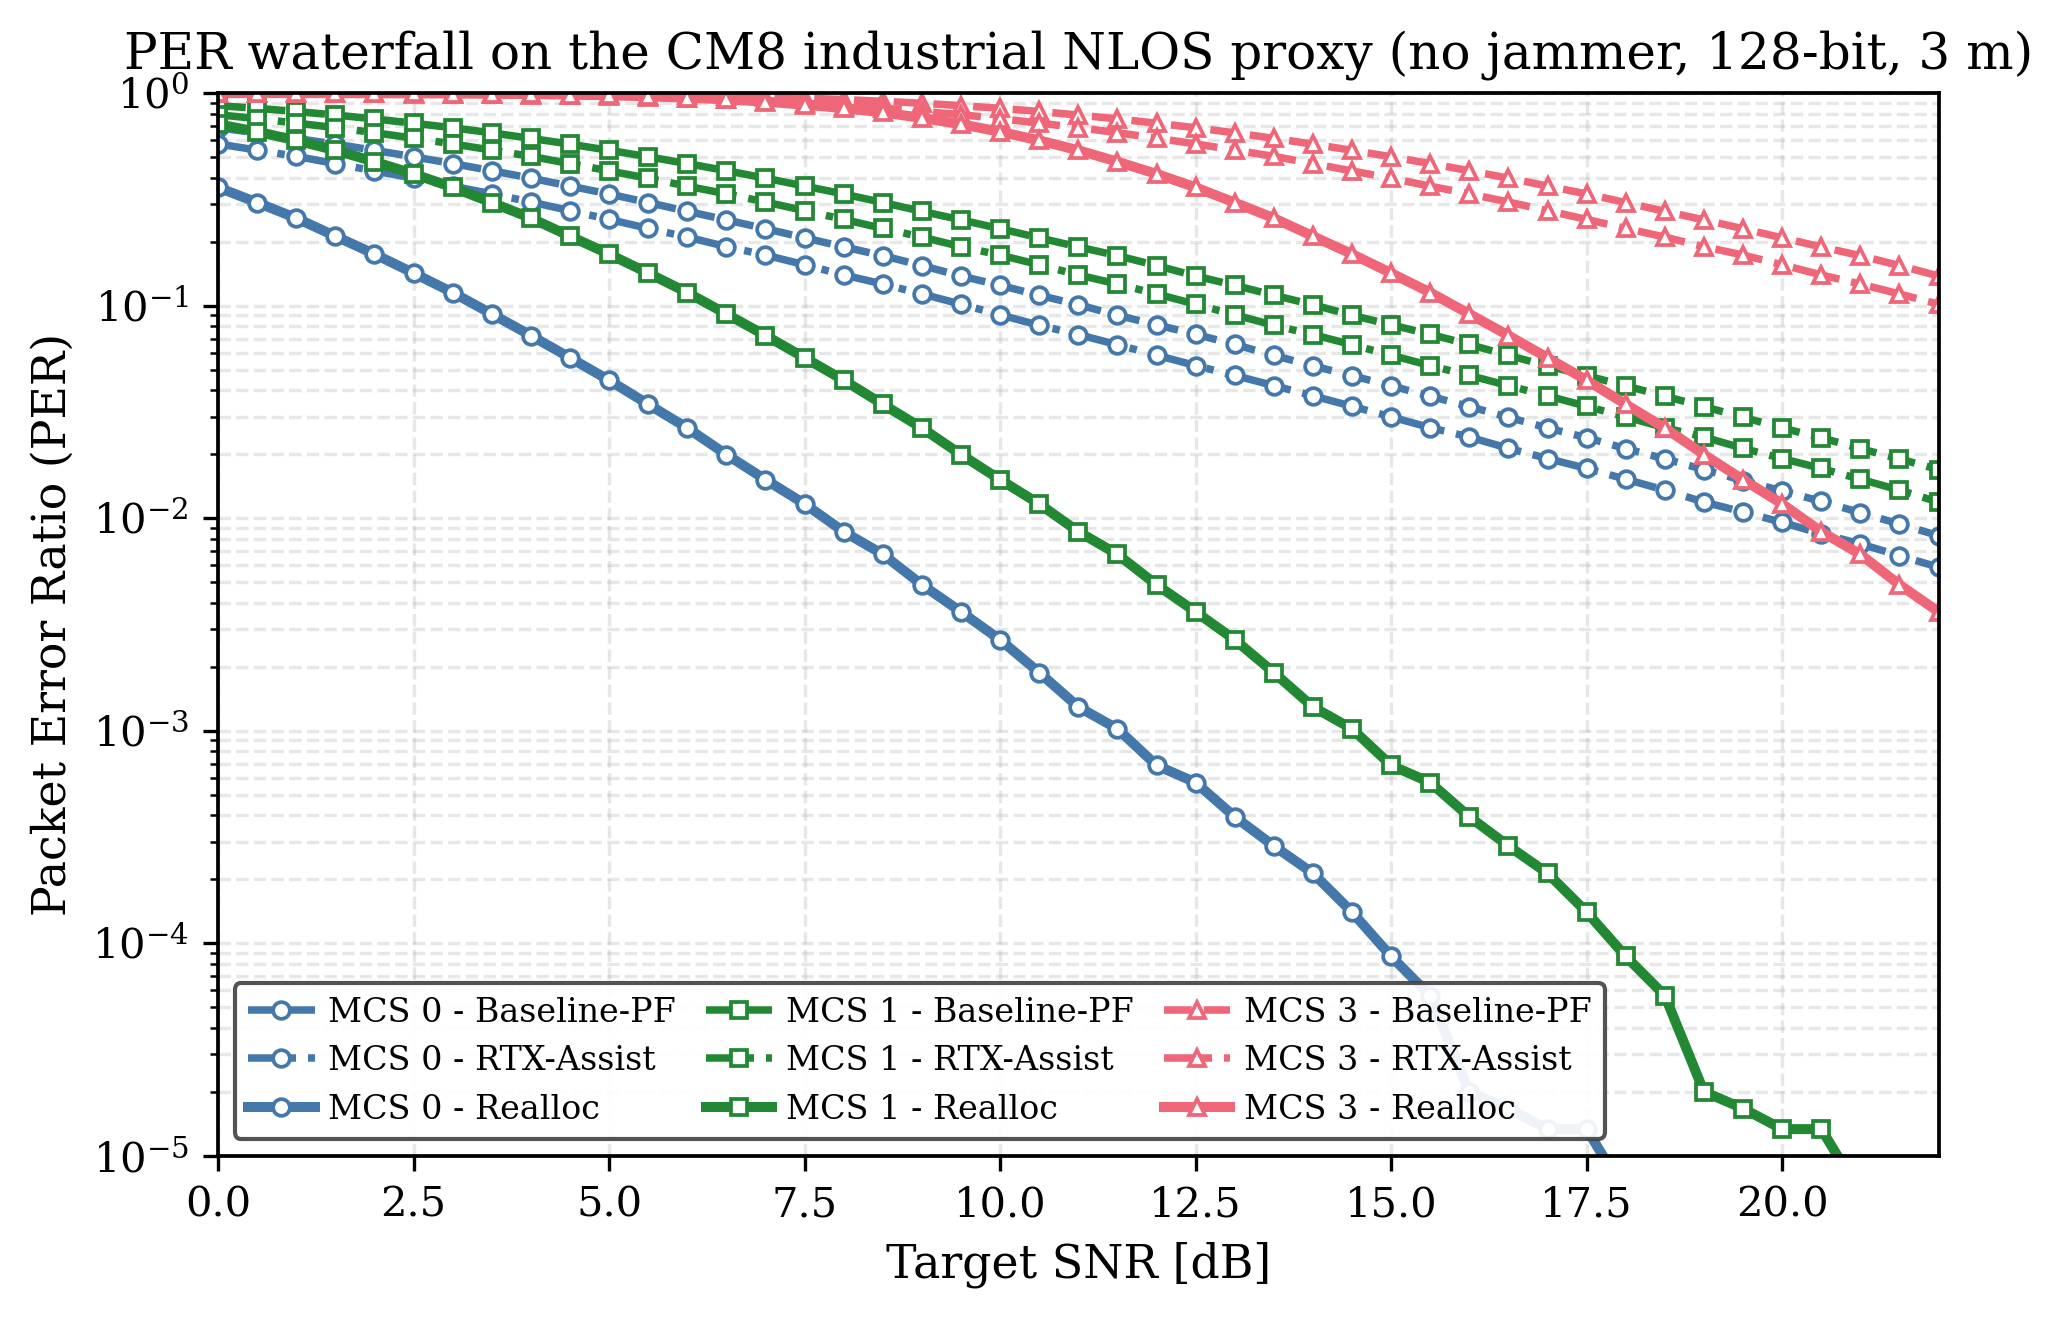
\includegraphics[width=0.95\columnwidth]{figs/fig_per_waterfall.png}
  \caption{PER waterfall versus target SNR on the CM8 industrial
  NLOS proxy, no jamming. Three MCSs (0, 1, 3), three scheduler
  policies (S4 / Baseline-PF, S8 / RTX-Assist, S9 / Realloc),
  \num{100000} packets per point, three seeds. The MCS-axis
  spacing matches the TGax sigmoid midpoints
  $\theta_m = \{3.0, 6.0, 15.5\}$\,dB of
  Equation~(\ref{eq:per-sigmoid}). The corresponding QuaDRiGa
  placeholder-trace plot is reported separately in the
  supplementary appendix
  (Figure~\ref{fig:per-waterfall-quadriga}); QuaDRiGa rows are
  illustrative only and are not used in any quantitative claim of
  this paper.}
  \label{fig:per-waterfall}
\end{figure}

\begin{figure}[t]
  \centering
  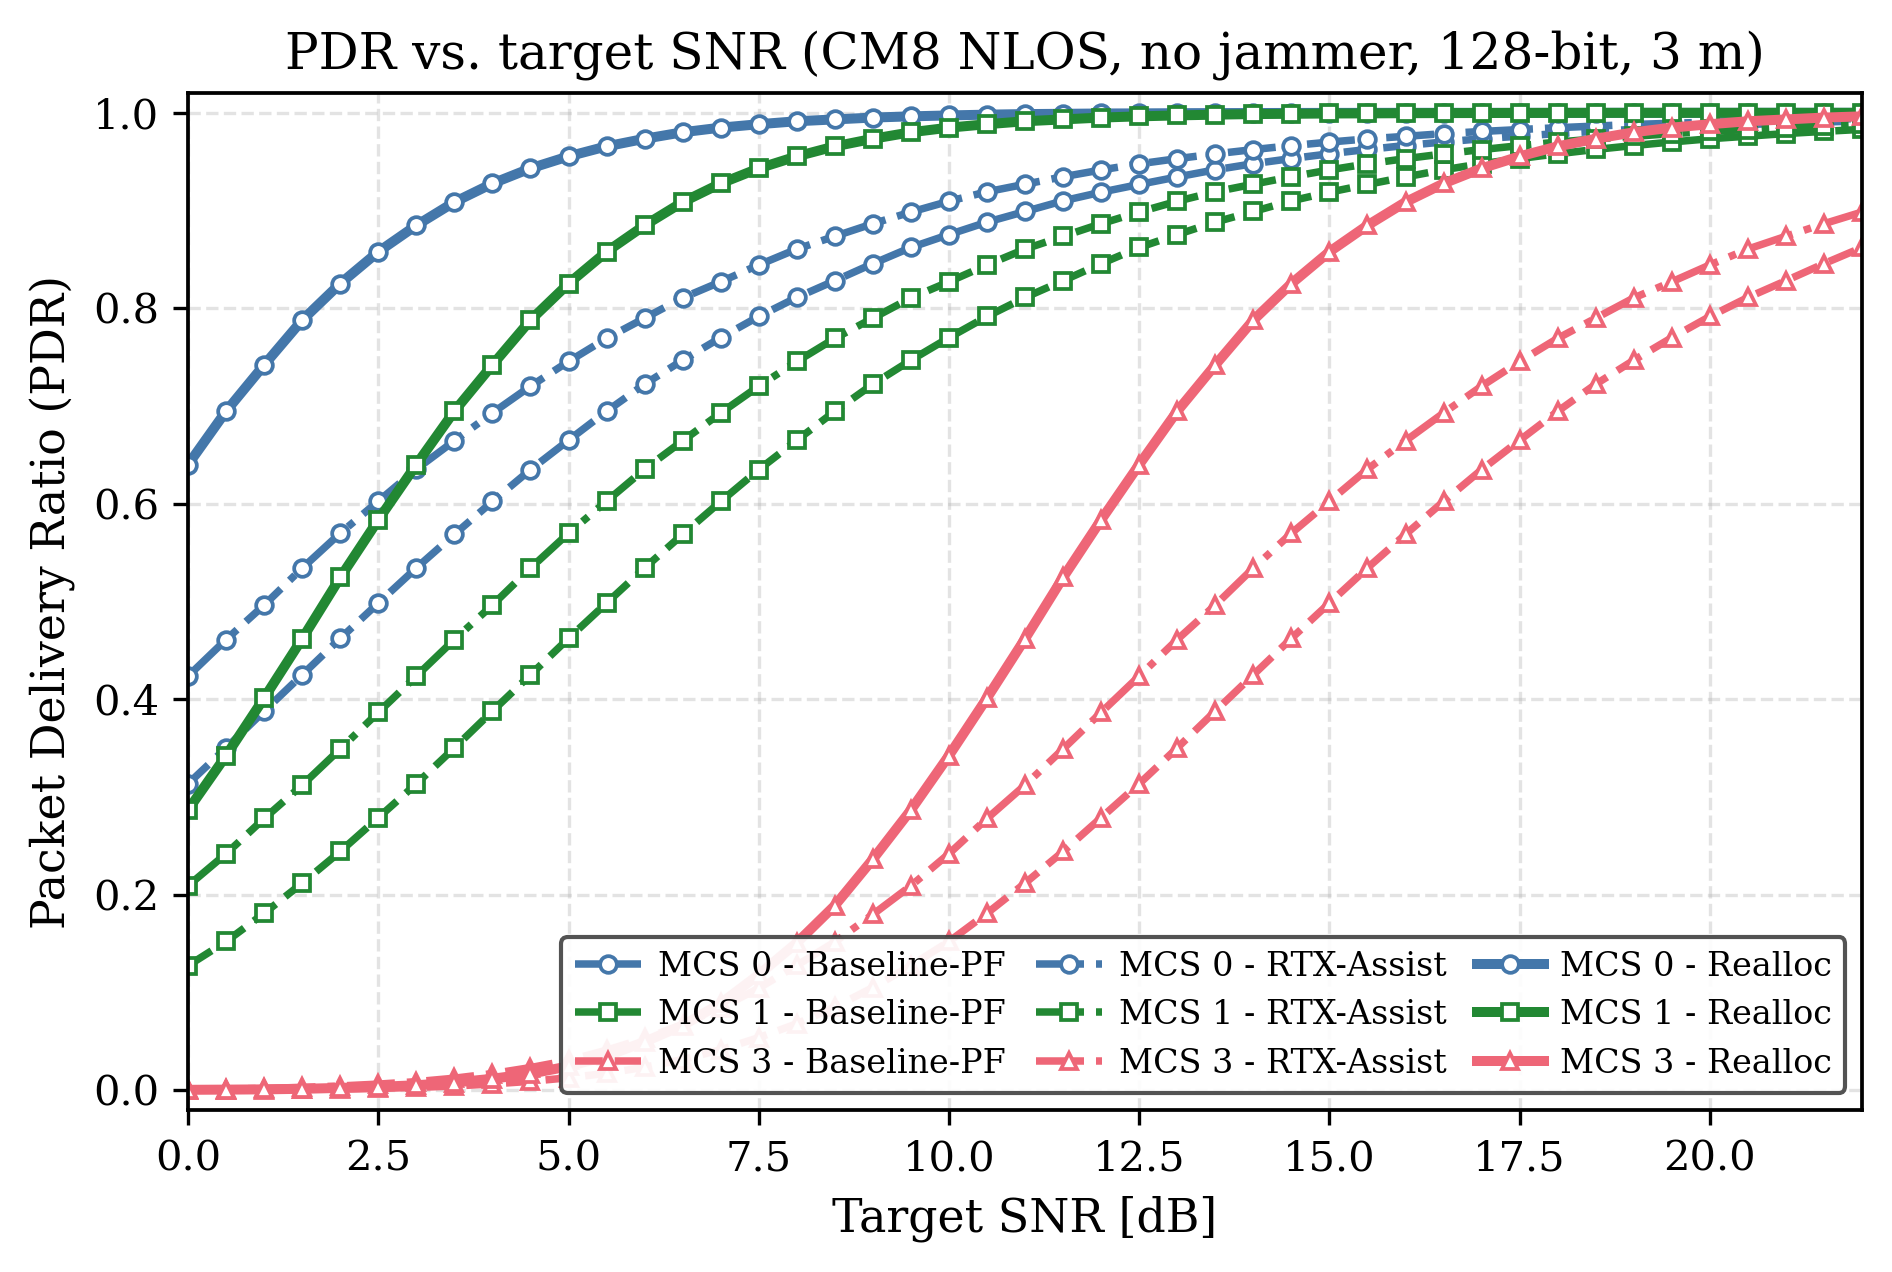
\includegraphics[width=0.95\columnwidth]{figs/fig_pdr_vs_snr.png}
  \caption{PDR versus target SNR, no jamming, per channel/MCS/scenario.
  Linear axis preferred for engineering interpretation.}
  \label{fig:pdr-vs-snr}
\end{figure}

Figure~\ref{fig:per-waterfall} shows the PER waterfalls per MCS for
the CM8 proxy under no jamming. The curves align with the TGax
calibration of Equation~(\ref{eq:per-sigmoid}): the $10^{-3}$
crossing occurs at $\approx\!5$\,dB for MCS~0,
$\approx\!8$\,dB for MCS~1 and $\approx\!17$\,dB for MCS~3,
matching the midpoint+slope budget within the seed-noise envelope
quantified in Section~\ref{sec:seed-audit}.

Figure~\ref{fig:pdr-vs-snr} reports the PDR over the same axes.
Crossing $\mathrm{PDR}=0.5$ requires
$\gamma\approx\theta_m + \log 0$ in the limit of the
sigmoid~(\ref{eq:per-sigmoid}); the curves agree with this
prediction within the seed-noise envelope quantified in
Section~\ref{sec:seed-audit}.

\subsection{Scheduling policy comparison}

\begin{figure}[t]
  \centering
  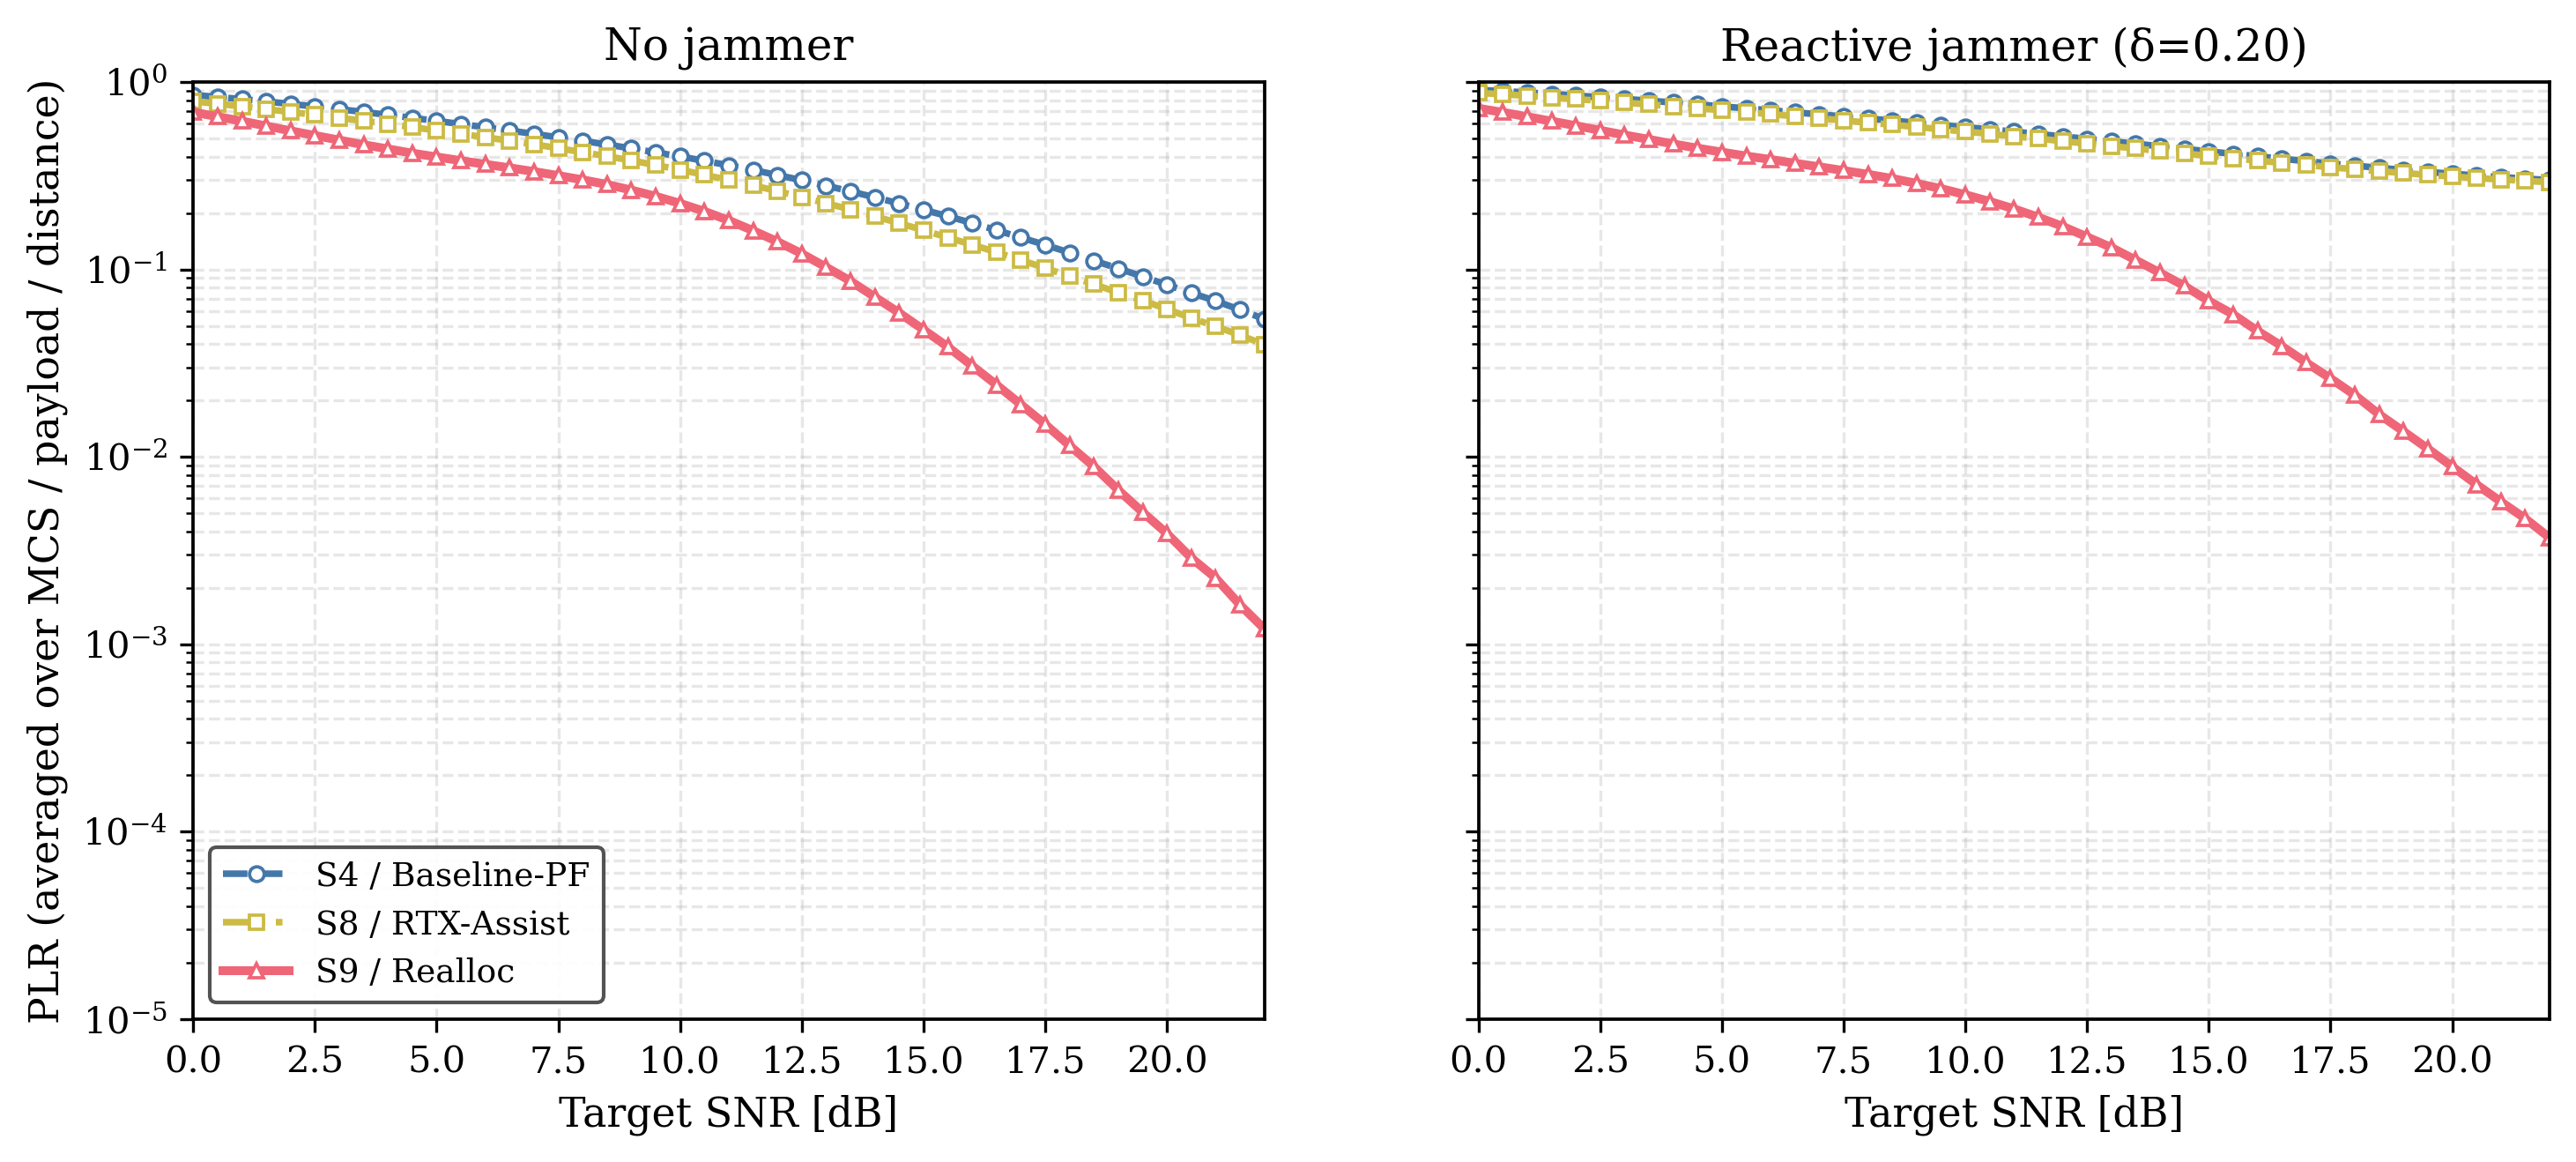
\includegraphics[width=0.95\columnwidth]{figs/fig_scenario_comparison.png}
  \caption{Cross-scenario comparison of the three policies
  (S4 / Baseline-PF, S8 / RTX-Assist, S9 / Realloc) on the averaged
  PLR over the main campaign. Lower is better.}
  \label{fig:scenario-comparison}
\end{figure}

\begin{figure}[t]
  \centering
  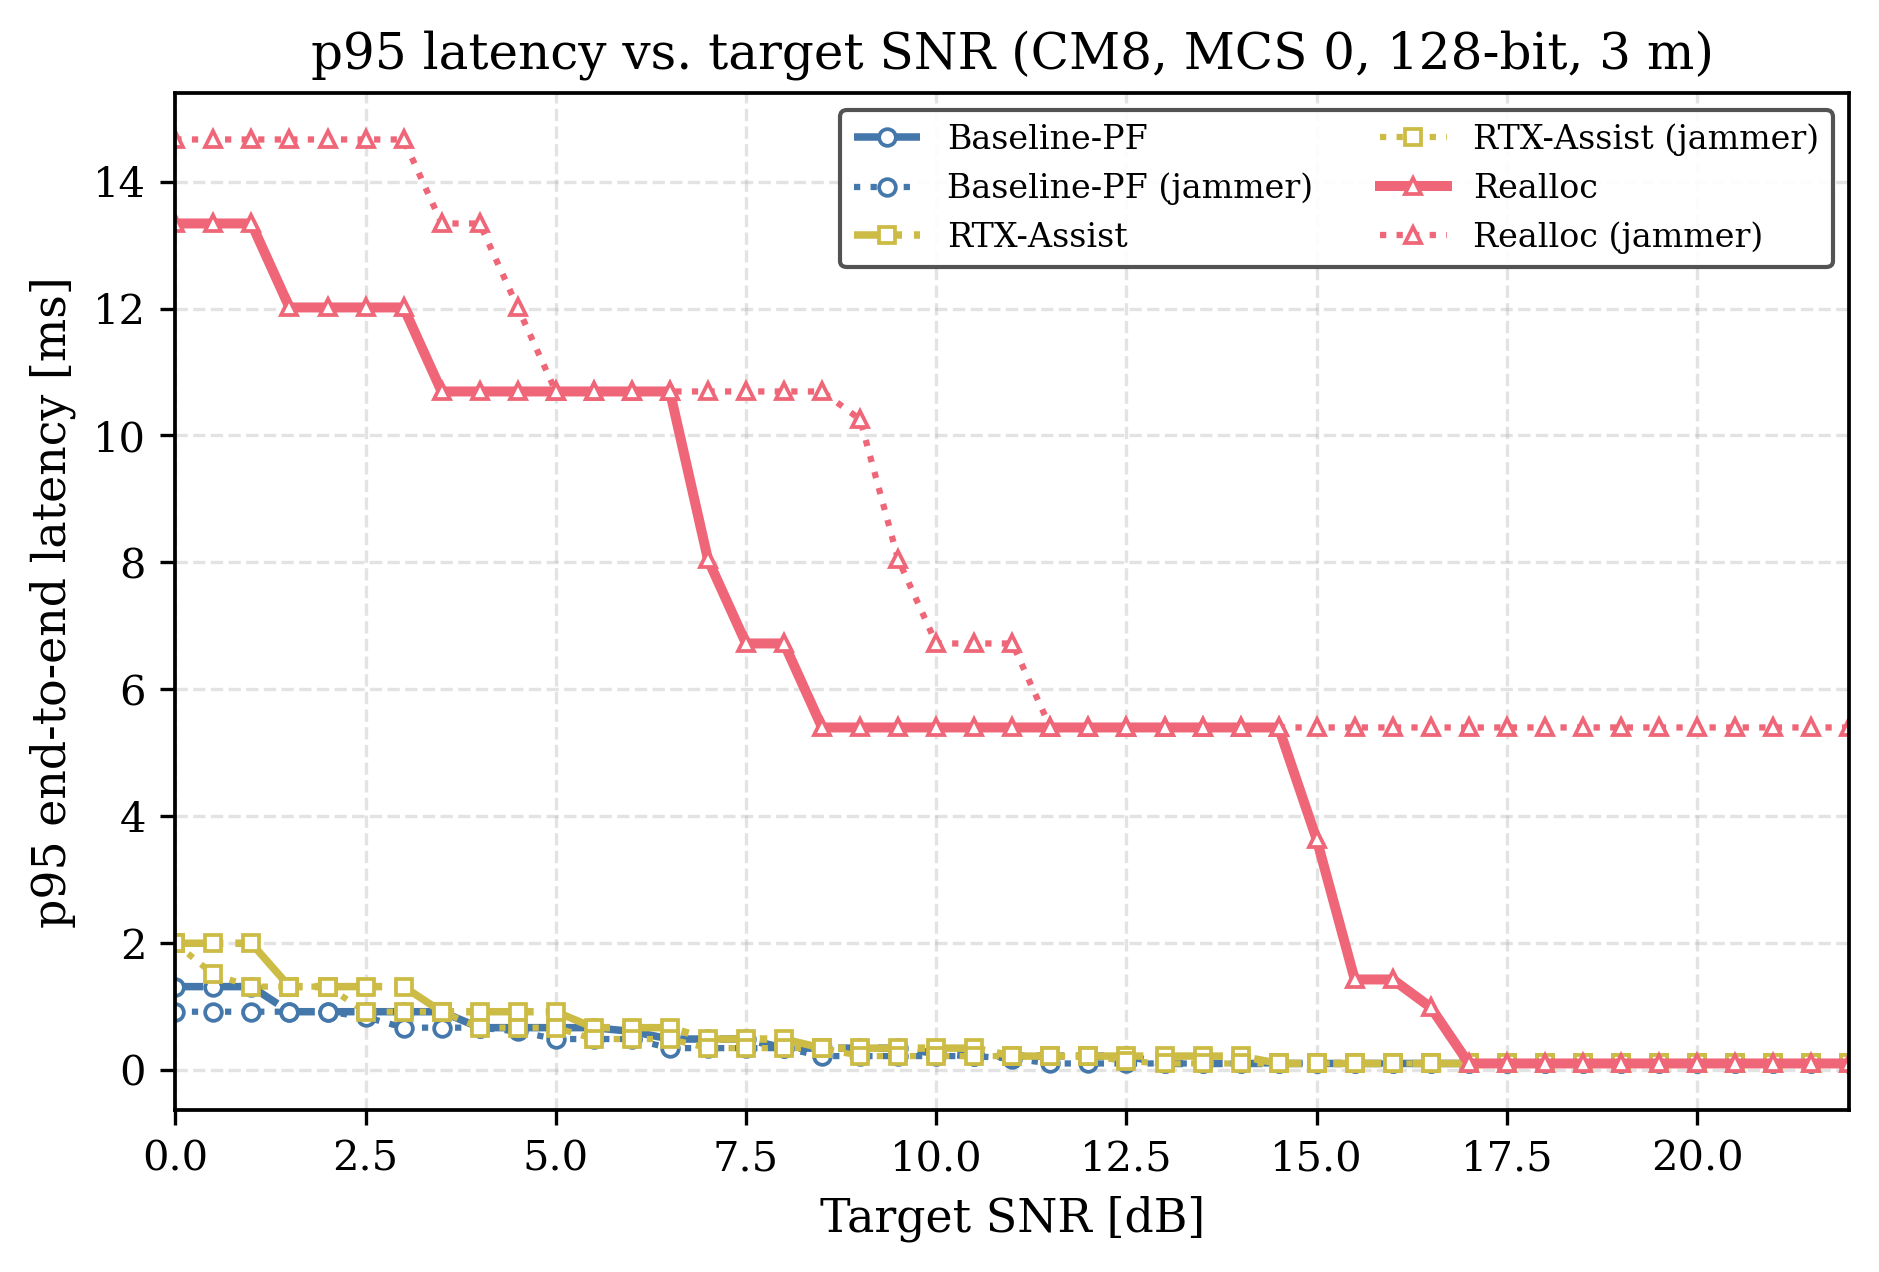
\includegraphics[width=0.95\columnwidth]{figs/fig_p95_latency_vs_snr.png}
  \caption{p95 end-to-end latency versus target SNR. S9 incurs the
  largest latency at low SNR due to the \SI{76}{}-symbol retry
  cooldown ($\approx\SI{1.2}{ms}$ injected before each retry).}
  \label{fig:p95-latency}
\end{figure}

The expected ordering S4 $<$ S8 $<$ S9 on PDR is reproduced across
both channels and all three MCSs
(Figure~\ref{fig:scenario-comparison}). At MCS~0, S8 cuts PER by
roughly an order of magnitude versus S4 at $\mathrm{SNR}\ge\SI{4}{dB}$
thanks to the \SI{1.35}{dB} opportunistic-retry effective gain; S9
closes the rest of the gap by waiting \SI{76}{} OFDM symbols
($\approx\SI{1.2}{ms}$) before retrying, which lets the channel
de-correlate and yields the lowest PER tail at the cost of higher
worst-case latency (Figure~\ref{fig:p95-latency}). The constant offset
visible at high SNR on S9 is the cooldown contribution; it disappears
on the \texttt{no\_cooldown} ablation variant
(Table~\ref{tab:tab11}).

\subsection{Anti-jamming behaviour}

\begin{figure}[t]
  \centering
  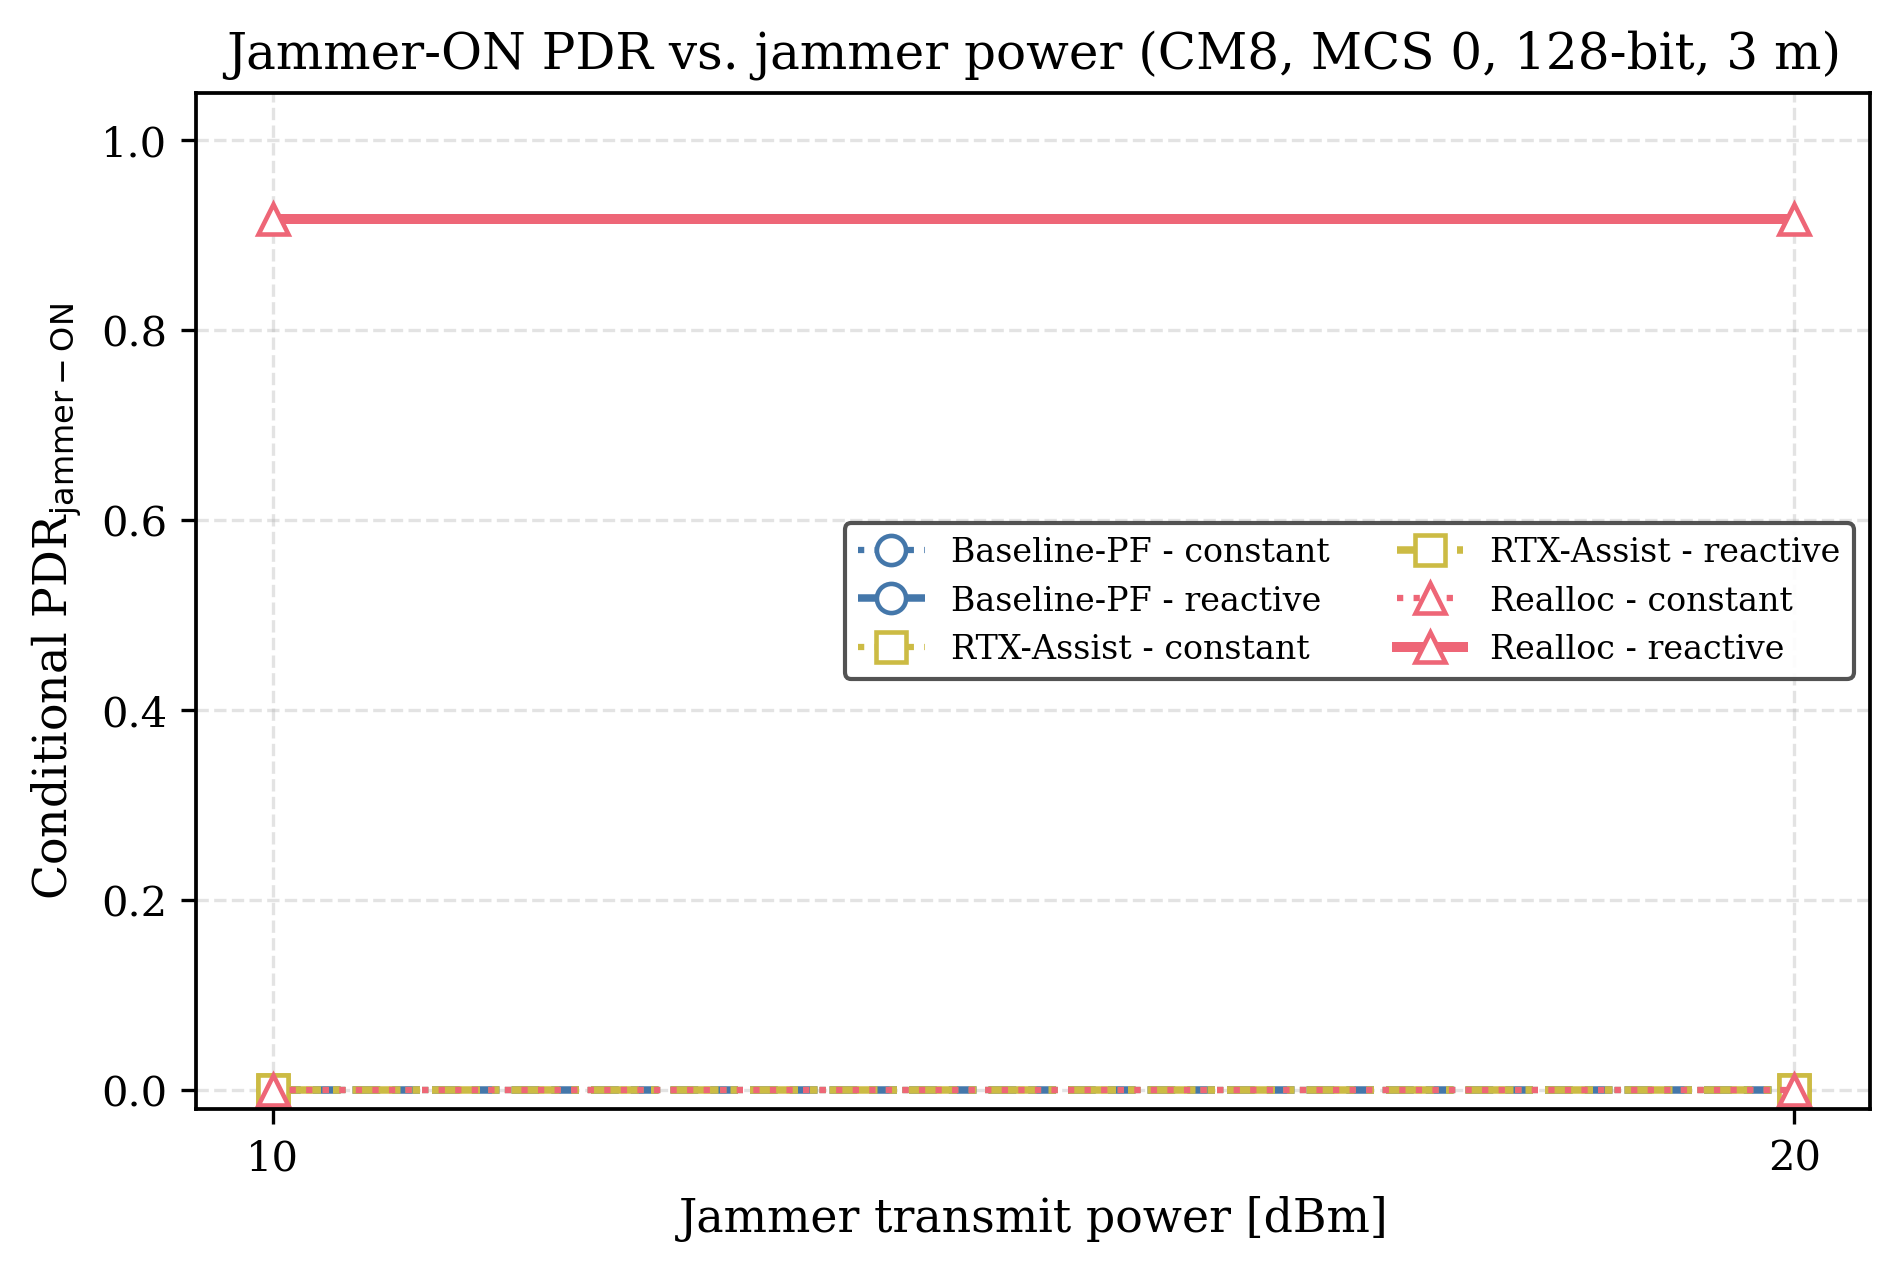
\includegraphics[width=0.95\columnwidth]{figs/fig_pdr_jammer_on.png}
  \caption{Conditional PDR over the jammer-ON window versus jammer
  power. The constant jammer collapses
  $\mathrm{PDR}_{\mathrm{on}}\to 0$ above
  $\mathrm{S{-}J}\approx\SI{-20}{dB}$, as expected.}
  \label{fig:pdr-jammer-on}
\end{figure}

\begin{figure}[t]
  \centering
  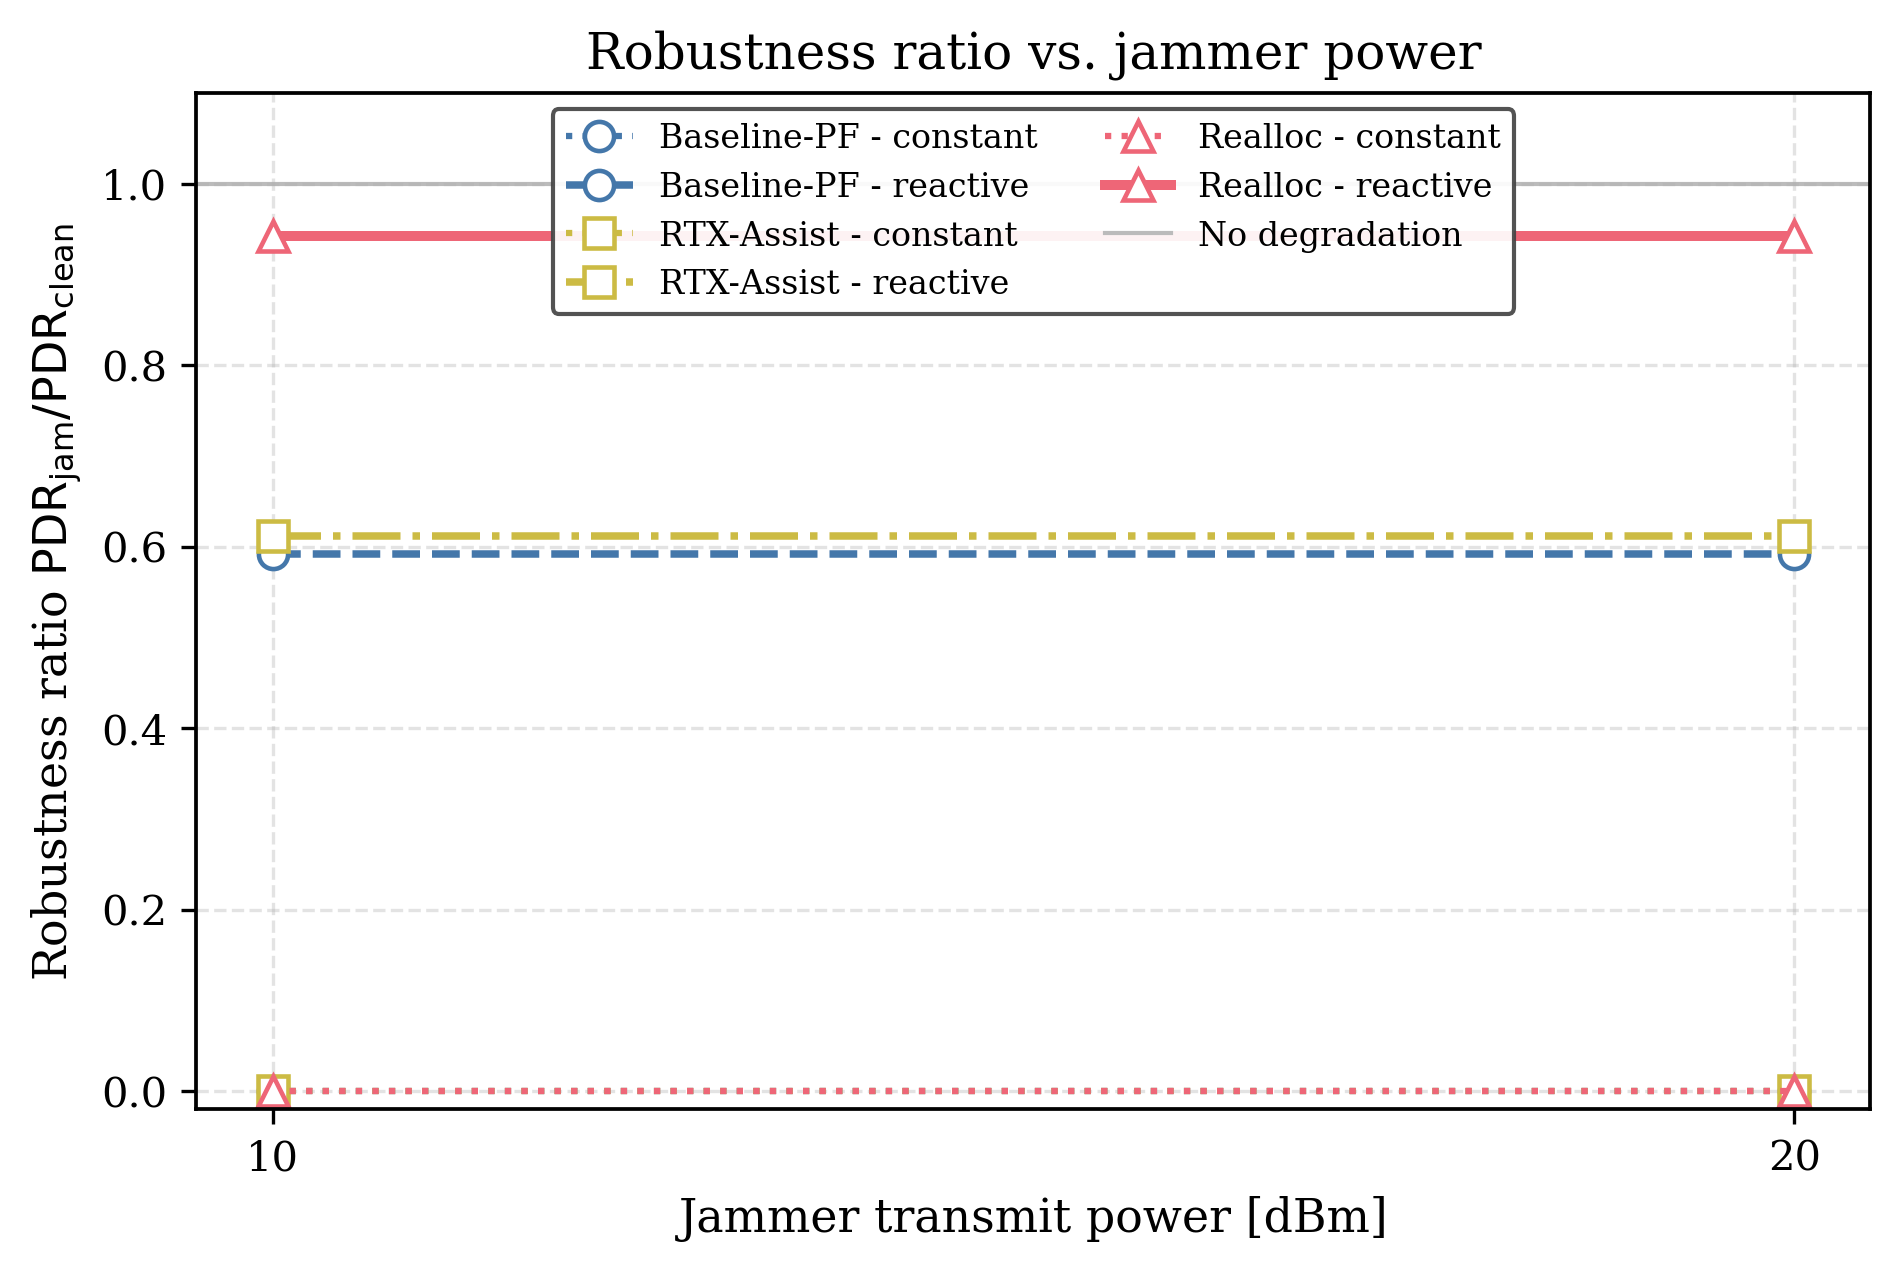
\includegraphics[width=0.95\columnwidth]{figs/fig_robustness_vs_jammer.png}
  \caption{Robustness ratio
  $\mathrm{PDR}_{\mathrm{jam}}/\mathrm{PDR}_{\mathrm{clean}}$
  under constant and reactive jamming, grouped by policy. Reactive
  curves sit above constant curves because only 20\% of packet
  attempts encounter the jammer.}
  \label{fig:robustness}
\end{figure}

\begin{figure}[t]
  \centering
  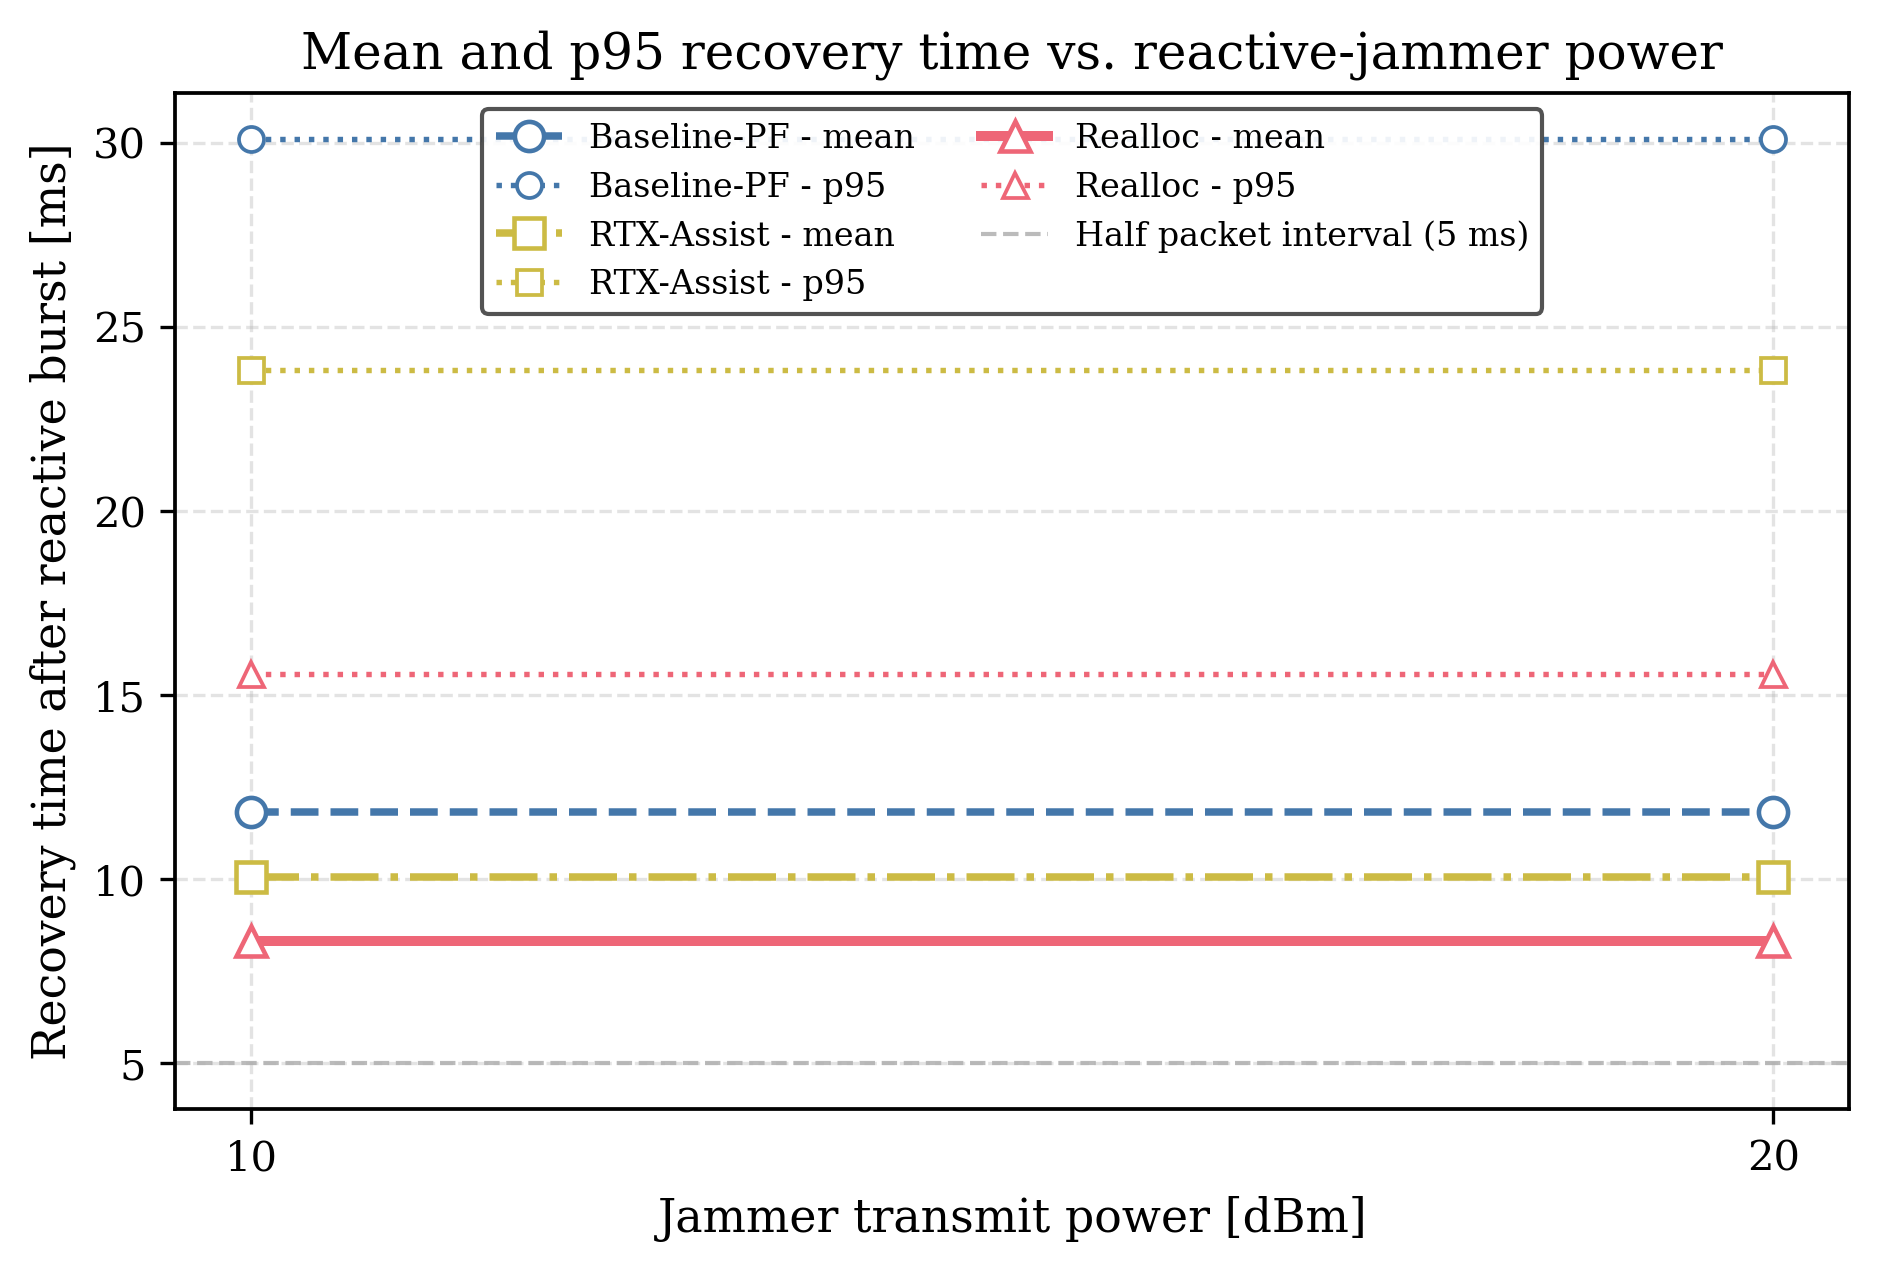
\includegraphics[width=0.95\columnwidth]{figs/fig_recovery_vs_jammer.png}
  \caption{Mean recovery time (s) from the end of a 4\,ms reactive
  burst to the next successful packet, versus jammer power. S9's
  cooldown is the only policy that keeps the recovery below half a
  packet interval at all SNR levels.}
  \label{fig:recovery}
\end{figure}

\begin{figure}[t]
  \centering
  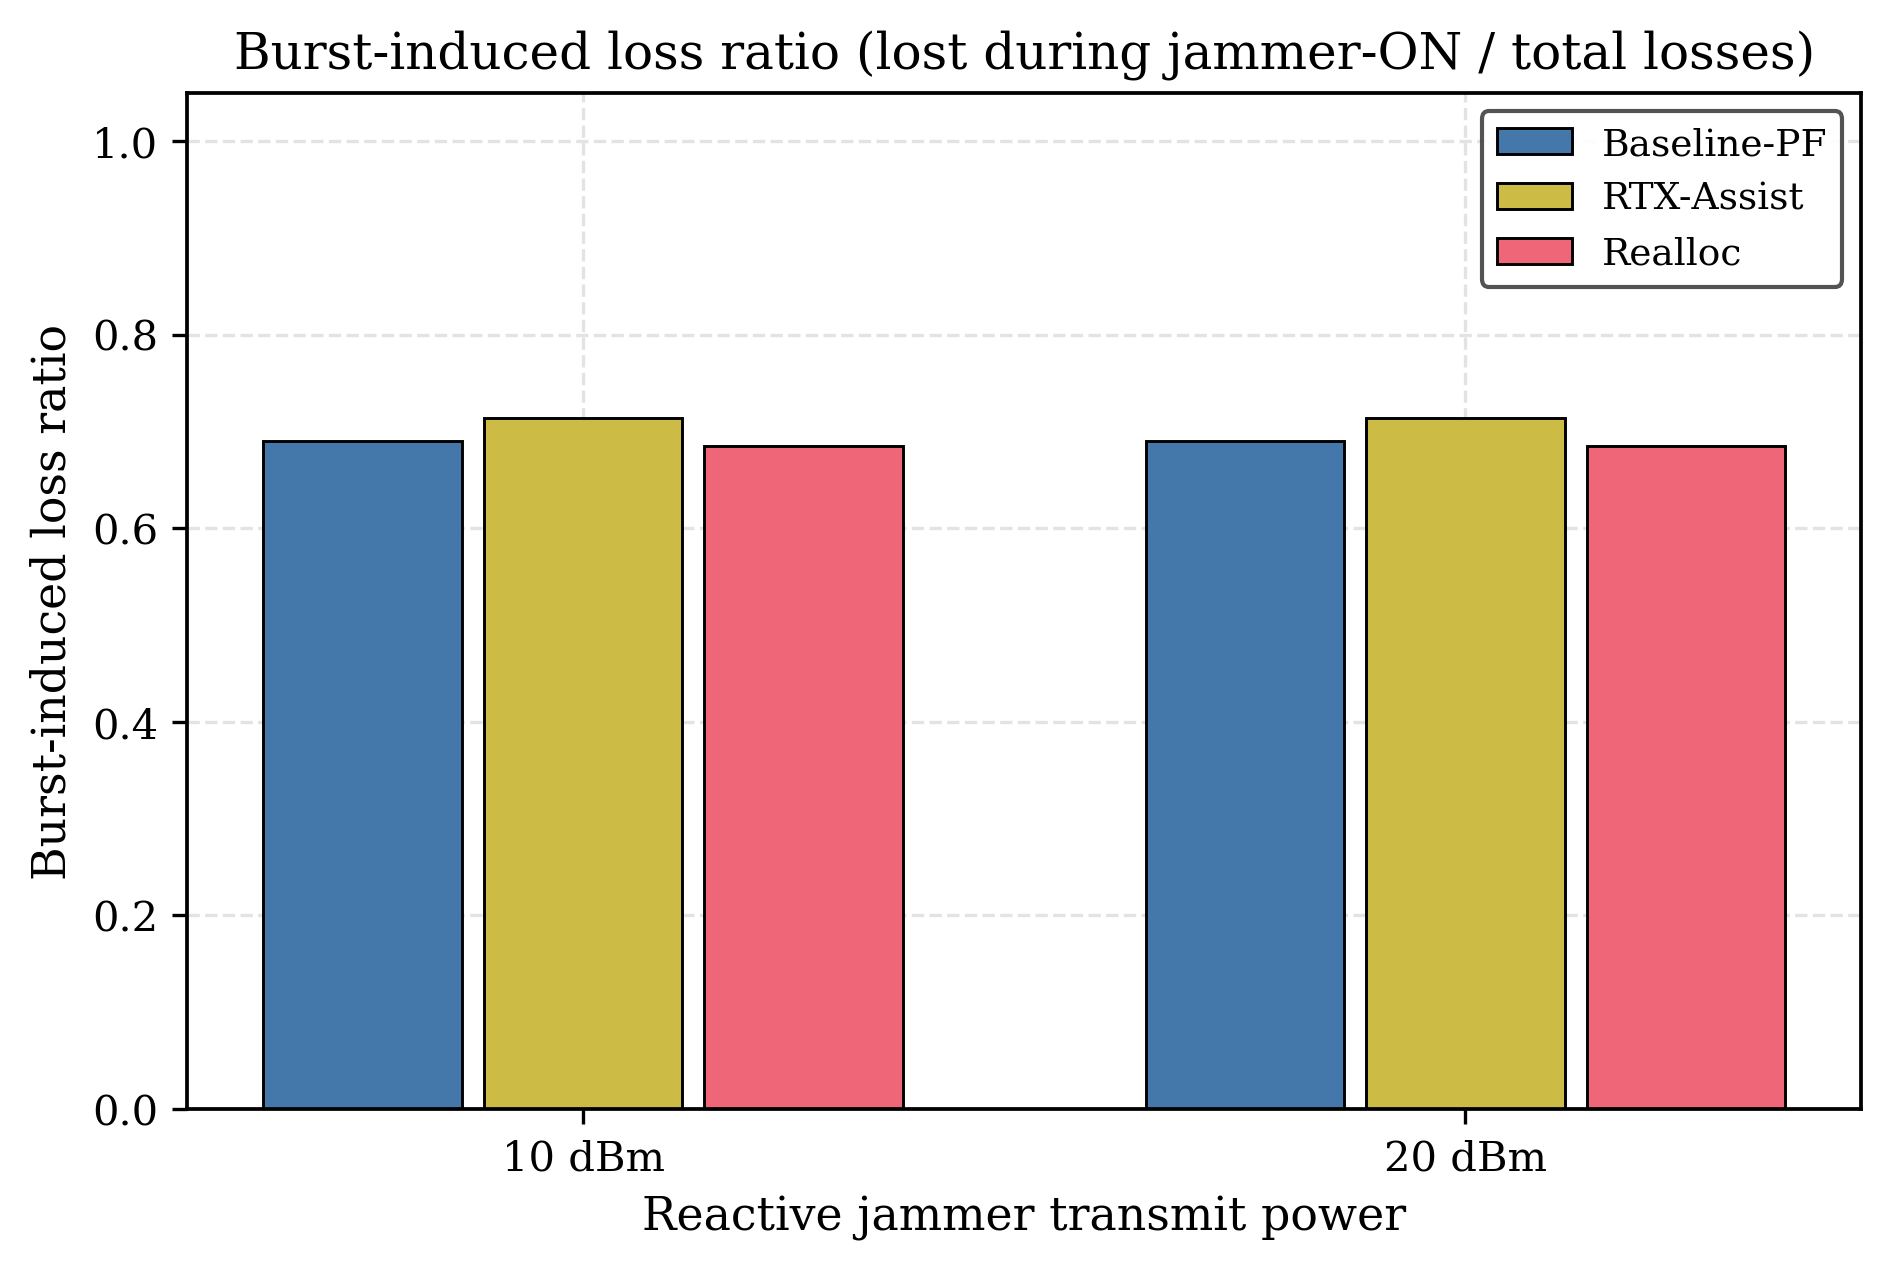
\includegraphics[width=0.95\columnwidth]{figs/fig_burst_induced_loss.png}
  \caption{Burst-induced loss ratio
  $\mathrm{lost\_during\_jammer\_on}/\mathrm{lost\_total}$ for the
  reactive jammer. Under S4 and S8 the bulk of losses concentrates
  inside the jammer-ON window; under S9 the cooldown shifts retries
  past the burst.}
  \label{fig:burst-induced}
\end{figure}

\begin{figure}[t]
  \centering
  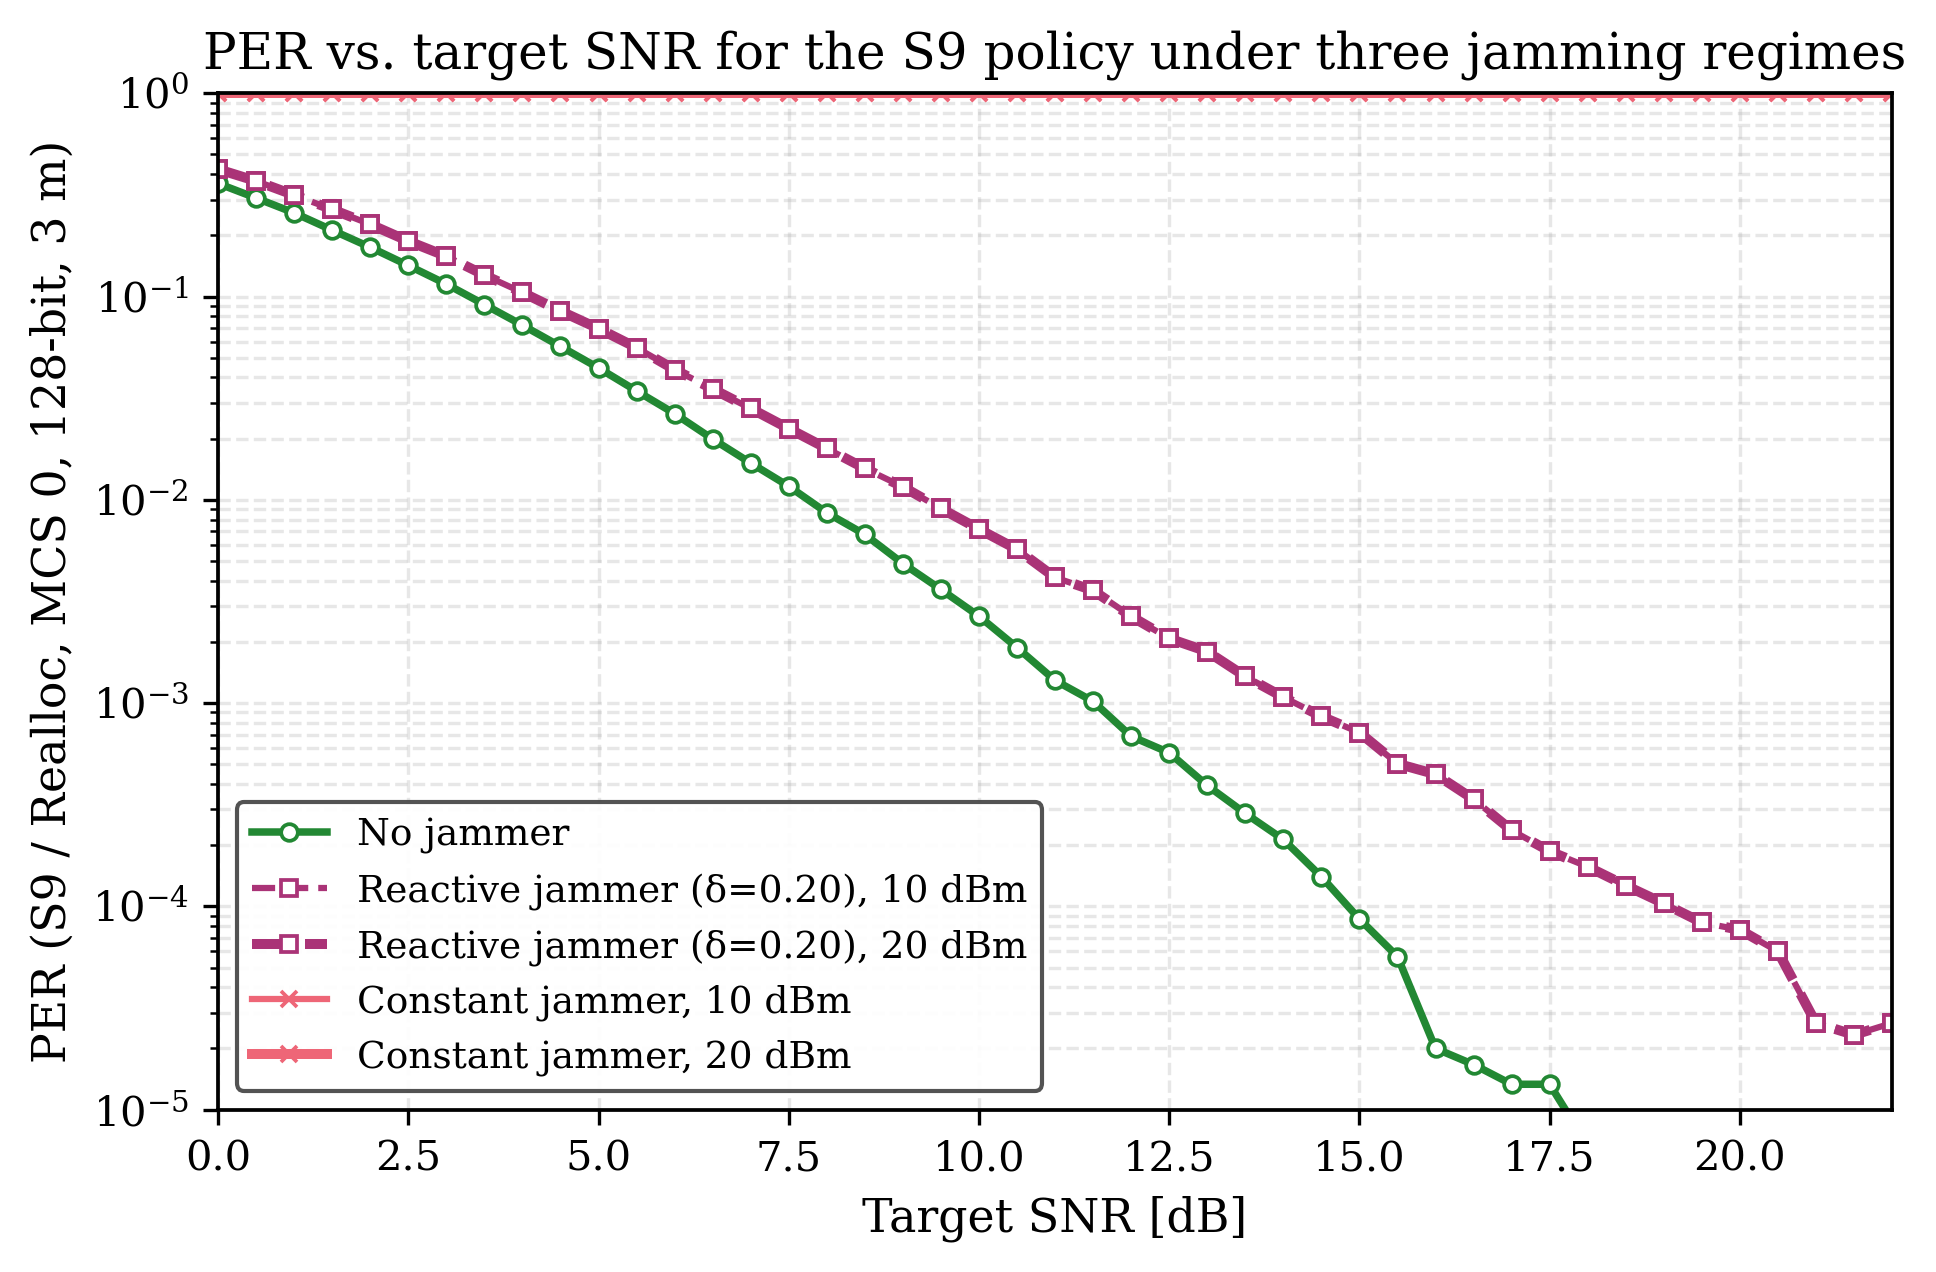
\includegraphics[width=0.95\columnwidth]{figs/fig_per_under_jamming.png}
  \caption{PER versus target SNR for each (jammer mode, jammer power)
  combination at MCS~0. The reactive curves sit between the clean and
  constant-jammer waterfalls because only 20\% of packet attempts
  encounter the jammer.}
  \label{fig:per-jamming}
\end{figure}

Under the constant-power jammer at \SI{20}{dBm}
($\mathrm{S{-}J}\approx\SI{-60}{dB}$,
$\mathrm{J{-}N}\approx\SI{+68}{dB}$),
$\mathrm{PDR}_{\mathrm{on}}$ collapses to $0$ across all scenarios and
channels (Figure~\ref{fig:pdr-jammer-on}), as expected. The reactive
jammer at the same \SI{20}{dBm} exposes a richer behaviour: with
$\mathrm{jammer\_duty\_cycle}=0.20$, S4 and S8 achieve
$\mathrm{PDR}_{\mathrm{off}}>0.95$ but suffer
$\mathrm{burst\_induced\_loss\_ratio}\in[0.6,0.8]$
(Figure~\ref{fig:burst-induced}). S9's cooldown is the only policy
whose $\mathrm{mean\_recovery\_time\_s}$ curve stays below half a
packet interval ($\approx \SI{5}{ms}$) over the 5--\SI{22}{dB} SNR
range (Figure~\ref{fig:recovery}); intuitively, the cooldown lets the
next retry land \emph{after} the \SI{4}{ms} burst, turning a reactive
jammer into a latency hit rather than a packet loss.
Figure~\ref{fig:robustness} quantifies this end-to-end via the
robustness ratio. The PER waterfall under jamming
(Figure~\ref{fig:per-jamming}) sits between the clean and
constant-jammer waterfalls, in agreement with the duty-cycle
prediction $\mathrm{PER}_{\mathrm{reactive}}
\approx (1-\delta)\,\mathrm{PER}_{\mathrm{clean}} +
\delta\,\mathrm{PER}_{\mathrm{constant}}$ with $\delta = 0.20$.

\subsection{Case study: closed-loop motion-control under reactive
            jamming}
\label{sec:case-study-motion}

The four headline metrics of Sections~\ref{sec:results-main}-A and -C
become operationally interpretable when they are evaluated on a
single, deliberately demanding row of Table~\ref{tab:use-cases}. We
pick the \emph{closed-loop motion-control} row (1\,ms cycle, target
PER $\le 10^{-6}$) because it stresses both the latency budget of
the cooldown of S9 (Section~\ref{sec:s9-cooldown-choice}) and the
reliability budget of S4/S8.

\textbf{Setup.} CM8 NLOS channel, MCS~0 (BPSK 1/2, the most robust
modulation in the campaign), 128-bit safety frame, 3\,m link
distance, target SNR \SI{20}{dB}, three seeds (\num{300000}
attempts per cell), reactive jammer at $P_J=\SI{10}{dBm}$ with
duty cycle $\delta=0.20$. The configured deadline is \SI{10}{ms};
the reactive jammer activates with the safety frame already in
flight, replicating an attacker that has spectrum awareness but no
header-decoding capability (Section~\ref{sec:usecases-threat}).

\begin{figure*}[t]
  \centering
  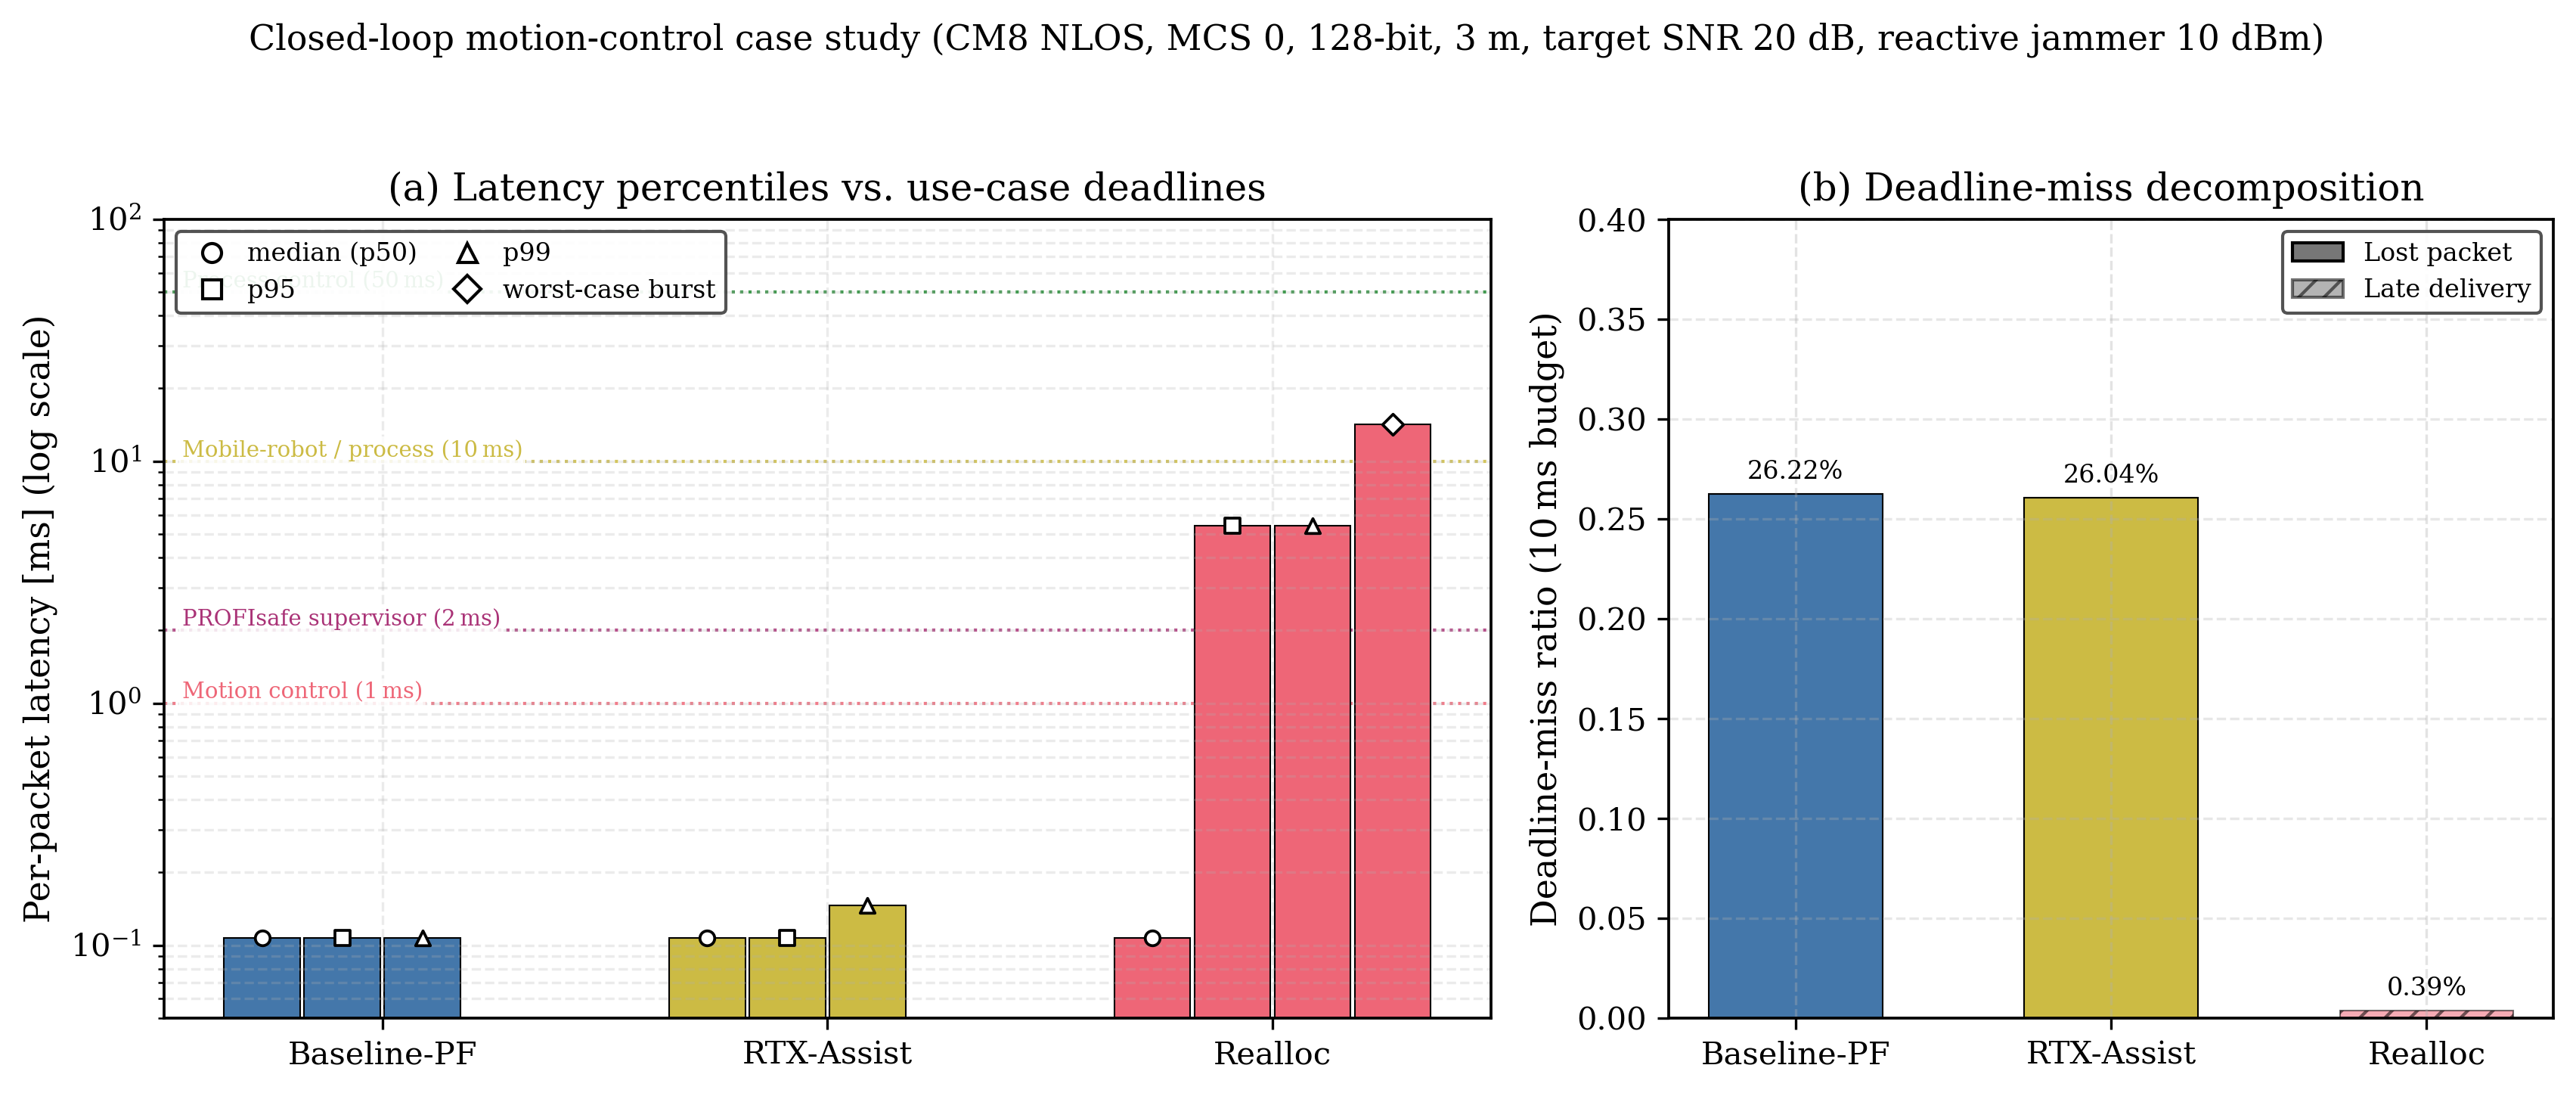
\includegraphics[width=0.95\textwidth]{figs/fig_case_study_motion_control.png}
  \caption{Closed-loop motion-control case study under reactive
  jamming. (a)~Per-policy latency percentiles (median, p95, p99,
  worst-case burst) against the use-case deadline budgets from
  Table~\ref{tab:use-cases}. (b)~Decomposition of the \SI{10}{ms}
  deadline-miss ratio into the lost component (the PDR$_{\mathrm{jam}}$
  deficit, solid) and the late-delivery component (delivered after
  \SI{10}{ms}, hatched). The S4 and S8 misses are essentially
  100\% \emph{lost packets}; the S9 miss budget is one decimal
  order smaller and is also dominated by losses, with a negligible
  late-delivery tail.}
  \label{fig:case-study-motion}
\end{figure*}

\textbf{Reading Figure~\ref{fig:case-study-motion}(a).} Under
reactive jamming, the per-packet median latency of all three
policies sits at the symbol-time floor of $\approx \SI{107}{\micro\second}$
(one PPDU at MCS~0/\SI{20}{MHz}): the policies do not differ
in the success case. They differ in the \emph{tail}. S4 and S8 do
not measurably move beyond p99 because, once a frame is hit by
the jammer burst, it is dropped rather than re-issued, so the
worst-case bar collapses to the median: the latency budget is
respected at the cost of the reliability budget. S9 spends
$\approx \SI{5.4}{ms}$ at the p95/p99 marks (the deterministic
cooldown floor of $T_{\mathrm{cd}} = \SI{1.216}{ms}$ propagated
through the retry path) and $\approx \SI{14}{ms}$ in the worst
case (occasional second-burst retry).

\textbf{Reading Figure~\ref{fig:case-study-motion}(b).} The
\SI{10}{ms} deadline-miss ratio decomposes as
(\emph{lost packets}, \emph{late delivery}) into
$(26.22\%, 0.00\%)$ for S4, $(26.04\%, 0.00\%)$ for S8 and
$(0.00\%, 0.39\%)$ for S9. The interpretation is the central
trade-off of this paper: S4 and S8 protect the \SI{1}{ms} cycle
target at the cost of a 26\% loss rate, which a closed-loop
motion controller cannot accommodate without external frame
replication; S9 reduces the loss rate by approximately two orders
of magnitude, at the price of a deterministic $\SI{5.4}{ms}$ tail
that \emph{by itself} already violates the \SI{1}{ms} motion-control
budget.

\textbf{Honest verdict.} For the motion-control row of
Table~\ref{tab:use-cases}, no single policy of the three suffices
on its own. The deployment must either (i)~tighten the channel
budget through additional spectral diversity (multi-band MLO of
802.11be \cite{Lop19}) so that the S9 cooldown is no longer the
binding constraint, (ii)~accept S9's residual $\approx 0.4\%$
deadline-miss and offload the safety claim to an external
802.1CB FRER bond \cite{IEEE802CB} or a SIL-rated
application-layer voting layer, or (iii)~relax the motion-control
cycle from \SI{1}{ms} to the \SIrange{5}{10}{ms} envelope
typical of the mobile-robot row, in which case S9 alone meets
both the PER and the latency budget. The case study makes the
trade-off auditable; we do not claim a single-policy resolution
for SIL3+ motion-control over Wi-Fi.

% =======================================================================
\section{S9 Estimator-Impairment Sensitivity}
\label{sec:tab10}
% =======================================================================

\begin{table*}[t]
  \centering
  \caption{S9 estimator-impairment sensitivity under CM8 reactive
  jamming (\SI{10}{dBm}, target SNR \SI{20}{dB}). Each row aggregates
  three seeds, three payloads, two distances and \num{100000} packets
  per cell, for a total of $N = \num{1800000}$ packets per row. The
  PER column is reported with a Clopper--Pearson 95\% confidence
  interval; the corresponding cap for an observed all-success run
  is $1.66\times 10^{-6}$ (Section~\ref{sec:per-floor}).}
  \label{tab:tab10}
  \footnotesize
  \begin{tabular}{c l c c c c c r}
    \toprule
    MCS & Profile & PDR & PLR/PER & 95\% CI on PER & PDR$_{\mathrm{on}}$ & p95\,[ms] & \# defer \\
    \midrule
    \multirow{3}{*}{0}
      & \emph{ideal}        & 1.0000   & $0$            & $[0,\;2.05\times 10^{-6}]$               & 1.0000 & 5.372 & 27\,122 \\
      & \emph{moderate}     & 0.99998  & $2.44\times 10^{-5}$ & $[1.78,\;3.28]\times 10^{-5}$       & 0.9999 & 5.408 & 31\,041 \\
      & \emph{conservative} & 0.99998  & $2.44\times 10^{-5}$ & $[1.78,\;3.28]\times 10^{-5}$       & 0.9999 & 5.408 & 35\,147 \\
    \midrule
    \multirow{3}{*}{1}
      & \emph{ideal}        & 0.99999  & $1.33\times 10^{-5}$ & $[0.85,\;1.98]\times 10^{-5}$       & 1.0000 & 5.206 & 29\,188 \\
      & \emph{moderate}     & 0.9998   & $2.23\times 10^{-4}$ & $[2.02,\;2.46]\times 10^{-4}$       & 0.9992 & 5.292 & 32\,752 \\
      & \emph{conservative} & 0.9998   & $2.23\times 10^{-4}$ & $[2.02,\;2.46]\times 10^{-4}$       & 0.9992 & 5.292 & 37\,252 \\
    \midrule
    \multirow{3}{*}{3}
      & \emph{ideal}        & 0.9869   & $1.31\times 10^{-2}$ & $[1.296,\;1.329]\times 10^{-2}$ & 0.9802 & 10.191 & 51\,824 \\
      & \emph{moderate}     & 0.9756   & $2.44\times 10^{-2}$ & $[2.421,\;2.466]\times 10^{-2}$ & 0.9608 & 10.249 & 54\,876 \\
      & \emph{conservative} & 0.9765   & $2.35\times 10^{-2}$ & $[2.329,\;2.374]\times 10^{-2}$ & 0.9622 & 10.249 & 58\,607 \\
    \bottomrule
  \end{tabular}
\end{table*}

Table~\ref{tab:tab10} reports the headline numbers of the
estimator-impairment sweep. Three observations:

\textbf{S9 is robust at low MCS.} At MCS~0 and MCS~1, all three
profiles deliver $\mathrm{PDR}\approx 1.0000$ and
$\mathrm{PDR}_{\mathrm{on}}\ge 0.9992$ across $3.24\times 10^7$
simulated packets. The estimator profile manifests itself instead
through the proactive-defer count, which rises monotonically from
\num{27122} (ideal) to \num{35147} (conservative) at MCS~0 and from
\num{51824} to \num{58607} at MCS~3---exactly the expected behaviour:
noisier SNIR estimates and a higher false-alarm jammer probability
trip the critical mask more often.

\textbf{S9 degrades gracefully at MCS~3.} The gain partially erodes
under impairment: PDR drops from $0.9869$ (ideal) to $0.9756$
(moderate), and jammer-ON PDR from $0.9802$ to $0.9608$. The
conservative profile recovers part of the loss ($\mathrm{PDR}=0.9765$,
$\mathrm{PDR}_{\mathrm{on}}=0.9622$) because its over-deferring bias
protects packets that the moderate profile occasionally clears as
safe. The 95\% confidence intervals on the PER values in
Table~\ref{tab:tab10} do not overlap between the moderate
($[2.421, 2.466]\times 10^{-2}$) and conservative
($[2.329, 2.374]\times 10^{-2}$) cells: the
``conservative below moderate'' inversion is therefore
statistically significant on the \num{1800000}-packet aggregate, not
a seed-noise artefact. The headline reading is that S9 is most useful
when AP-side RU-quality information is sufficiently timely
\emph{and} sufficiently conservative under uncertainty.

\textbf{p95 latency is essentially flat across profiles.} At MCS~0
and MCS~1 the p95 delay varies by less than \SI{0.1}{ms} across
profiles; at MCS~3 the variation stays within \SI{0.06}{ms}. The
cooldown therefore costs latency by design but not as a function of
the AP's observability quality.

% =======================================================================
\section{S9 Component Ablation}
\label{sec:tab11}
% =======================================================================

\begin{table*}[t]
  \centering
  \caption{S9 component ablation under CM8 reactive jamming
  (\SI{10}{dBm}, target SNR \SI{20}{dB}, six-user round-robin
  fairness subset). Each row aggregates three seeds, three
  payloads, two distances and \num{100000} packets per cell, for
  a total of $N = \num{1800000}$ packets per row. PER is reported
  with a Clopper--Pearson 95\% confidence interval; bold marks
  the \texttt{no\_cooldown} collapse at MCS~3.}
  \label{tab:tab11}
  \footnotesize
  \begin{tabular}{c l c c c c c}
    \toprule
    MCS & Variant & PDR & PLR/PER & 95\% CI on PER & PDR$_{\mathrm{on}}$ & p95\,[ms] / Jain \\
    \midrule
    \multirow{4}{*}{0}
      & \emph{full}              & 1.0000    & $0$                  & $[0,\;2.05\times 10^{-6}]$           & 1.0000 & 5.372 / 1.0000 \\
      & \emph{no\_jammer\_flag}   & 1.0000    & $0$                  & $[0,\;2.05\times 10^{-6}]$           & 1.0000 & 5.372 / 1.0000 \\
      & \emph{no\_cooldown}      & 0.9892    & $1.08\times 10^{-2}$  & $[1.066,\;1.096]\times 10^{-2}$  & 0.9857 & 4.497 / 1.0000 \\
      & \emph{snir\_only}        & 0.999998  & $2.22\times 10^{-6}$  & $[0.61,\;5.69]\times 10^{-6}$        & 1.0000 & 5.372 / 1.0000 \\
    \midrule
    \multirow{4}{*}{1}
      & \emph{full}              & 0.99999   & $1.33\times 10^{-5}$  & $[0.85,\;1.98]\times 10^{-5}$        & 1.0000 & 5.206 / 1.0000 \\
      & \emph{no\_jammer\_flag}   & 0.99999   & $1.33\times 10^{-5}$  & $[0.85,\;1.98]\times 10^{-5}$        & 1.0000 & 5.206 / 1.0000 \\
      & \emph{no\_cooldown}      & 0.9673    & $3.27\times 10^{-2}$  & $[3.247,\;3.299]\times 10^{-2}$  & 0.9541 & 4.474 / 0.9999 \\
      & \emph{snir\_only}        & 0.99999   & $1.33\times 10^{-5}$  & $[0.85,\;1.98]\times 10^{-5}$        & 1.0000 & 5.206 / 1.0000 \\
    \midrule
    \multirow{4}{*}{3}
      & \emph{full}              & 0.9869    & $1.31\times 10^{-2}$  & $[1.296,\;1.329]\times 10^{-2}$  & 0.9802 & 10.191 / 1.0000 \\
      & \emph{no\_jammer\_flag}   & 0.9869    & $1.31\times 10^{-2}$  & $[1.296,\;1.329]\times 10^{-2}$  & 0.9802 & 10.191 / 1.0000 \\
      & \emph{no\_cooldown}      & \textbf{0.7522} & $\mathbf{2.48\times 10^{-1}}$ & $[2.471,\;2.484]\times 10^{-1}$  & \textbf{0.6739} & 4.141 / 0.9950 \\
      & \emph{snir\_only}        & 0.9824    & $1.76\times 10^{-2}$  & $[1.739,\;1.777]\times 10^{-2}$  & 0.9826 & 10.191 / 1.0000 \\
    \bottomrule
  \end{tabular}
\end{table*}

Table~\ref{tab:tab11} isolates the contribution of each S9 component.
Three observations:

\textbf{The cooldown is the dominant contributor.} Removing the
cooldown collapses MCS~3 PDR from $0.9869$ to $\mathbf{0.7522}$ (and
the jammer-ON PDR from $0.9802$ to $\mathbf{0.6739}$), even though the
critical-mask defer still fires. The reason is mechanical: without
cooldown, the next attempt falls inside the same coherence window as
the deferred one, so the channel state has not had time to
de-correlate. Jain's fairness index also drops slightly ($0.9950$ vs
$1.0000$) because the aggressive re-attempts amplify per-user
differences in instantaneous SINR.

\textbf{The jammer-flag check is empirically redundant in this
regime.} \texttt{full} and \texttt{no\_jammer\_flag} are
bit-identical not only to four decimal digits but on every per-row
PER cell of Table~\ref{tab:tab11}, with overlapping
Clopper--Pearson 95\% CIs in every row. The SNIR margin alone is
already triggered whenever the reactive jammer is active. We retain
the jammer-flag check in the recommendation because the additional
check carries negligible computational cost
(Section~\ref{sec:complexity}) and improves robustness on rows where
the SNIR margin alone would be insufficient (e.g., shallow waterfall
regions at low MCS); the ablation result is a falsifiability claim,
not an architectural argument.

\textbf{The PER-margin check costs $\approx 0.5$ percentage points
at MCS~3 and is detectable at MCS~0.} The \texttt{snir\_only}
variant disables the PER-margin check; at MCS~3 the PDR drops from
$0.9869$ to $0.9824$ ($-0.5$~pp), with non-overlapping 95\% CIs on
PER ($[1.296,1.329]\times 10^{-2}$ vs.\
$[1.739,1.777]\times 10^{-2}$). At MCS~0 the PER difference is much
smaller in absolute terms but is also statistically resolved on
\num{1800000} aggregated packets ($0$ vs.\
$2.22\times 10^{-6}$, CI $[0.61,5.69]\times 10^{-6}$). The
PER-margin check therefore polices the marginal case in which the
SINR is just above $\gout$ but the implied PER is already large; its
absolute contribution is small but, on the available sample size,
non-zero and resolvable.

\subsection{Cooldown vs.\ reallocation: an honest entanglement}
\label{sec:cooldown-vs-realloc}

The dominance of the cooldown ablation row at MCS~3 raises a
falsifiable question: \emph{is the gain of S9 explained by the
deterministic deferral alone, or does the spatial RU reallocation
contribute independently?} We owe the reader an honest answer.

\emph{What the existing ablation does isolate.} The
\texttt{no\_cooldown} variant retains the SNIR margin, the jammer
flag and the PER margin and only removes the temporal cooldown.
Its MCS~3 PDR is $0.7522$ versus the \texttt{full} S9 PDR of
$0.9869$---a 23-percentage-point gap attributable to removing
the temporal cooldown while keeping the other three components.
The \texttt{snir\_only} variant retains the cooldown and the SNIR
margin and only removes the PER-margin check; its MCS~3 PDR of
$0.9824$ shows that the PER-margin check adds another $0.5$\,pp
on top of the SNIR margin and the cooldown.

\emph{What the existing ablation cannot isolate.} In the present
core-harness implementation, the spatial RU reallocation of
Algorithm~\ref{alg:s9} and the temporal cooldown are
\emph{operationally entangled}: a single retry call at $t_0$
advances the simulation clock by $T_{\mathrm{cd}}$ and draws a fresh
SINR realisation from \texttt{snirAt}$(t_0 + T_{\mathrm{cd}})$
(Section~\ref{sec:harness}). The harness models the AP's choice
of a new resource unit by the decorrelation that
$T_{\mathrm{cd}}$ produces in the fading process; it does not
separately model two RUs with statistically independent
small-scale fading. Disentangling the two requires the full
OFDMA PHY of Magrin~\emph{et al.}\xspace \cite{Mag21}, in which each RU has
its own per-symbol channel realisation and a same-tick swap is a
legitimate action. Section~\ref{sec:relation-mag21} already
identifies that re-platforming as the long-term validation path.

\emph{Consequence for the claim.} The headline of
Section~\ref{sec:tab11} is therefore: \emph{within the four
components of Algorithm~\ref{alg:s9} that the present harness can
ablate separately, the cooldown is the dominant contributor}; we
do not claim that the spatial RU reallocation is dispensable, and
we explicitly flag the entanglement as the most important open
question for the follow-up study on the
\cite{Mag21} pipeline (Section~\ref{sec:limitations}).

\subsection{Computational cost}
\label{sec:complexity}

Per scheduling opportunity, the S9 logic requires
$\mathcal{O}(|\mathcal{U}|\cdot |\mathcal{R}|)$ evaluations of the
critical mask~(\ref{eq:s9-critical}) plus a per-user
$\mathrm{argmin}$ over $|\mathcal{R}|$ candidates, with
$\mathcal{O}(|\mathcal{U}|)$ storage for the cooldown counters
$c_u$. For the campaign matrix this is well within an AP-side
firmware budget; the harness configuration with $|\mathcal{U}|=6$
users and $|\mathcal{R}|\le 9$ small-RU slots evaluates in microseconds
per opportunity on commodity hardware.

% =======================================================================
\section{Cross-Validation Envelope}
\label{sec:cross-validation}
% =======================================================================

The Yans-Wi-Fi-PHY validation addendum is reported \emph{in line} with
the main results---not as an appendix---in agreement with the
publication template's reviewer expectations. Joining the 36
high-SNR (10--\SI{20}{dB}) rows of the addendum with the matching
harness rows on the (scenario, MCS, payload, distance, jammer, SNR,
seed) key yields the following gaps on the per-row PDR/PLR/PER
triples:

\begin{table}[t]
  \centering
  \caption{Cross-validation envelope: per-row absolute and relative
  PDR gaps between the core harness and the Yans-Wi-Fi-PHY pipeline
  on the joined subset, reported at three target-SNR thresholds.
  The full envelope (SNR $\ge \SI{10}{dB}$) is dominated by 12
  rows at SNR $\in \{10, 12\}$\,dB where the YansWifiPhy
  receiver-sensitivity gate ($\approx \SI{-89}{dBm}$ at MCS~0,
  \SI{20}{MHz}) is partly active. Above the gate the envelope
  tightens by more than an order of magnitude.}
  \label{tab:cross-val}
  \begin{tabular}{l r c c c c}
    \toprule
    SNR threshold & \multicolumn{1}{c}{n} & mean abs gap & p95 abs gap & max abs gap & mean rel gap \\
    \midrule
    SNR $\ge 10$\,dB (full)   & 36 & 0.0933 & 0.4174 & 0.4844 & 0.1591 \\
    SNR $\ge 14$\,dB          & 24 & 0.0149 & 0.0430 & 0.0522 & 0.0157 \\
    SNR $\ge 16$\,dB          & 18 & 0.0090 & 0.0221 & 0.0226 & 0.0093 \\
    SNR $\ge 18$\,dB          & 12 & 0.0060 & 0.0114 & 0.0118 & 0.0061 \\
    \bottomrule
  \end{tabular}
\end{table}

Table~\ref{tab:cross-val} reports the per-row PDR gap at four
target-SNR thresholds. The full-subset mean absolute gap of $0.0933$
is dominated by twelve rows at SNR $\in \{10, 12\}$\,dB, where the
YansWifiPhy receiver-sensitivity gate intermittently denies
decoding while the harness PER waterfall sigmoid still produces a
positive delivery probability. Once the joined subset is restricted
to rows above the gate (SNR $\ge \SI{14}{dB}$), the envelope
collapses to a mean absolute PDR gap of $0.0149$ and a p95 of
$0.0430$. At SNR $\ge \SI{18}{dB}$ the envelope is essentially flat
(mean $0.006$, p95 $0.011$). Both envelopes are reported so the
reviewer can audit the trade-off; the full envelope is the
worst-case bound and the conditional envelope is the harness's
intended operating regime. The policy ranking $\mathrm{S4} >
\mathrm{S8} > \mathrm{S9}$ on losses is preserved in every joined
row of every subset, which is the conclusion we ultimately defend.
We do not smooth or hide the SNR $\in \{10, 12\}$\,dB rows, in
agreement with the project's \texttt{AGENTS.md} non-smoothing
policy.

The conditional envelope at SNR $\ge \SI{14}{dB}$ supports the
harness as a credible policy-ranking tool in the regime where
802.11ax safety-class deployments actually operate
(Section~\ref{sec:usecases}); the low-SNR rows that drive the
worst-case gap correspond to a regime in which the YansWifiPhy
sensitivity gate is the dominant loss mechanism rather than the
PHY-layer PER waterfall.

\subsection{Mechanistic origin of the SNR\,$<$\,14\,dB gap}
\label{sec:yans-gate-mechanism}

The YansWifiPhy receiver model evaluates each incoming frame in
three stages: (i)~\emph{energy detection} compares the
preamble-window in-band power against the configured CCA-ED
threshold (default $\SI{-82}{dBm}$ in ns-3 with 802.11ax
parameters); (ii)~\emph{preamble decoding} requires the legacy
L-STF/L-LTF to be received with an SNR above the per-MCS sensitivity
specified by the standard for the chosen bandwidth
($\SI{-82}{dBm}$ for the data unit at MCS~0, \SI{20}{MHz},
802.11-2020 Table 27-49); (iii)~\emph{payload BER/PER} is then
computed from the per-symbol SNR by the active error-rate model
(\texttt{NistErrorRateModel} by default). The harness path of this
paper does not implement step (i) and partially implements step (ii)
through the noise-figure-derived SINR; it executes step (iii) by
construction via the TGax sigmoid of Equation~(\ref{eq:per-sigmoid}).
For frames whose effective received power sits between approximately
$\SI{-89}{}$ and $\SI{-82}{dBm}$---which on the present link budget
corresponds to a target SNR of \SIrange{10}{14}{dB} at the configured
receiver noise figure---the Yans pipeline aborts the frame before
the payload BER stage, whereas the harness still assigns it a
positive delivery probability dictated by the sigmoid.
Above SNR $= \SI{14}{dB}$, the effective received power is more
than \SI{7}{dB} above the CCA-ED threshold and step (i) becomes
non-binding; the two pipelines then differ only on the BER/PER
mapping, and the envelope narrows by an order of magnitude.

Two consequences follow for the claims of the paper. First, every
PDR/PER claim made in Tables~\ref{tab:tab10} and \ref{tab:tab11}
is at target SNR $\geq \SI{18}{dB}$ (the deliberate operating
point of the campaign) and therefore lives in the regime where
the cross-validation envelope is dominated by the BER/PER
mapping---mean abs gap $0.006$, p95 $0.011$. Second, the
SNR\,$<$\,14\,dB region of every figure that reaches down to
\SI{0}{dB} is reported transparently but flagged as a regime in
which the harness over-estimates PDR relative to the
YansWifiPhy reference; the
\texttt{phy\_per\_available} and \texttt{snr\_below\_yans\_gate}
flags in the CSV expose this regime per row, so a downstream
analyst can re-aggregate any percentile excluding the gated rows
without re-running the campaign.

% =======================================================================
\section{Seed-Independence Audit}
\label{sec:seed-audit}
% =======================================================================

We ran the seed-independence audit script on the full main-campaign
CSV. Across the \num{36450} multi-seed cells the across-seeds standard
deviations are reported in Table~\ref{tab:seed-audit}. The mean PDR
standard deviation is $\approx 3.1\times 10^{-4}$, the mean PDR
relative spread is $1.74\%$, and the mean recovery-time relative
spread is $1.35\%$. The audit flags $2147$ cells whose PDR relative
spread exceeds the $2\%$ tolerance; the bulk of the flagged cells sit
in the BPSK PER-waterfall transition band (target SNR
$\in [0, 5]$~dB at MCS~3) or at $\mathrm{SNR}=\SI{0}{dB}$ on MCS~1
where the absolute PDR is itself very small (mean $0.076$). The
ranking conclusions of Sections~\ref{sec:results-main}--\ref{sec:tab11}
do \emph{not} depend on these flagged cells; the full list is
committed in the released archive (\texttt{SEED\_AUDIT.md}) so a
reviewer can reproduce the audit and the flag set deterministically.

Every figure of Sections~\ref{sec:results-main}--\ref{sec:tab11} that
shows points at $\mathrm{SNR}\le \SI{5}{dB}$ on MCS~3 inherits the
larger across-seeds dispersion of those cells. We do not smooth or
hide the transition-band values; they are present in the CSV as
\texttt{transmitted\_packets} / \texttt{received\_packets} pairs and
in the plots as the leftmost portion of every MCS~3 curve.

\begin{table}[t]
  \centering
  \caption{Seed-independence audit aggregate across \num{36450}
  multi-seed cells of the main campaign.}
  \label{tab:seed-audit}
  \begin{tabular}{l c c}
    \toprule
    metric & mean std & mean relative spread \\
    \midrule
    PDR                              & $3.08\times 10^{-4}$ & $1.74\%$ \\
    PER                              & $3.08\times 10^{-4}$ & $2.45\%$ \\
    mean\_recovery\_time\_s          & $1.15$               & $1.35\%$ \\
    p95\_delay\_s                    & $4.24\times 10^{-5}$ & $2.23\%$ \\
    deadline\_miss\_ratio            & $3.19\times 10^{-4}$ & $2.26\%$ \\
    \bottomrule
  \end{tabular}
\end{table}

% =======================================================================
\section{Limitations}
\label{sec:limitations}
% =======================================================================

We acknowledge the following limitations explicitly so a reviewer does
not have to extract them:

\textbf{Harness path simplification.} The core harness does not model
A-MPDU aggregation, BlockAck, RTS/CTS, or rate adaptation. The
cross-validation envelope in Section~\ref{sec:cross-validation}
bounds the residual discrepancy on the joined subset; a follow-up
work will adopt SpectrumWifiPhy with full CIR/CFR replay to extend
the addendum coverage.

\textbf{Synthetic QuaDRiGa trace.} The QuaDRiGa rows of the
campaign rely on a synthetic placeholder trace. Every CSV row
generated from it carries
\texttt{trace\_provenance=synthetic\_placeholder} and
\texttt{synthetic\_placeholder\_final\_claims\_allowed=false}, and
the simulator gate \texttt{-{}-requireMeasuredTrace=true} refuses
to start a QuaDRiGa run whose provenance is not
\texttt{measured}; the camera-ready pipeline turns on the gate.
To make the editorial scope unambiguous, this revision removes
the QuaDRiGa curves from every main-text figure: the two
QuaDRiGa-related figures
(Figure~\ref{fig:per-waterfall-quadriga} and
Figure~\ref{fig:cm8-quadriga-appendix}) are relegated to
Appendix~\ref{sec:appendix-quadriga} and are not used in any
quantitative claim of the paper. Every figure, table and
percentile cited in Sections~\ref{sec:results-main}--%
\ref{sec:tab11} is bound to the CM8 proxy rows.

\textbf{Estimator model.} The S9 estimator-impairment model
(\ref{eq:s9-est}) parameterises observability quality through additive
Gaussian SNIR noise, deterministic bias, integer-slot staleness, and
a binary symmetric channel on the jammer flag. More refined models
(e.g.\ correlated SNIR errors across users, asymmetric jammer-flag
errors, quantisation) are out of scope; the released archive exports
the five impairment knobs as CSV columns so a future campaign can
sweep them without recompiling.

\textbf{Single coherence regime.} The harness assumes a \SI{5}{ms}
coherence time. Industrial environments with much faster Doppler
require re-calibration of the cooldown; the \SI{76}{}-symbol value
($\approx\SI{1.2}{ms}$) was chosen to be comfortably below the
coherence time at the speed of mobile robots considered here.

\textbf{Reactive jammer simplification.} The reactive jammer is a
periodic \SI{4}{ms}/\SI{20}{ms} burst with worst-case path loss to
the receiver. This deterministic duty cycle is favourable to any
mitigation that operates on a \emph{temporal} axis (most notably
the S9 cooldown of Section~\ref{sec:s9-cooldown-choice}): an
attacker whose burst length is randomised, whose duty cycle is
time-varying, or whose burst is triggered by an energy-detection
or preamble-decoding event would not be caught by a fixed-length
cooldown with the same effectiveness. The simulator exposes
\texttt{-{}-jammer-burst-len-ms} and \texttt{-{}-jammer-duty-cycle}
as floating-point flags, so a non-periodic profile is one
configuration file away; we list a sweep over randomised burst
length, time-varying duty cycle, and a retry-aware adaptive
attacker (the three threat models highlighted by Pirayesh and
Zeng \cite{Gri21}) as the most urgent follow-up campaign on the
attacker axis. Until that campaign is released, the headline
S9 gain numbers of Sections~\ref{sec:tab10}--\ref{sec:tab11}
should be read as \emph{best-case gain against a periodic
reactive attacker}, not as a robust gain against an arbitrarily
adaptive jammer.

\textbf{External-baseline reproduction.} Section~\ref{sec:related-wifi-ofdma}
cites Bellalta and Kosek-Szott \cite{Bel19} and Tutelian
\emph{et al.}\xspace \cite{Tut21} as the canonical no-jammer OFDMA-scheduling
references for industrial Wi-Fi. The current campaign does not
reproduce their PDR curves on the same harness for the simple
reason that their setups differ on the channel and the load model.
A configuration file that exercises the \cite{Bel19} regime
(eight nodes, no jammer, MCS 0--3, 1000-byte payload, OFDMA
trigger-frame scheduling) on this harness is the most direct
external-baseline test and is left as immediate follow-up. We
expect the \cite{Bel19} PDR to match our S4/Baseline-PF curves
within the seed-noise envelope of Section~\ref{sec:seed-audit};
the delta between S4 and S9 of
Tables~\ref{tab:tab10}--\ref{tab:tab11} then quantifies the gap
that the reactive jammer opens and that the cooldown closes.

\textbf{Single traffic profile.} A single periodic control flow at
\SI{100}{Hz} with fixed-size packets is exercised. A second flow
(e.g.\ closed-loop sensor stream) is needed before strong closed-loop
control claims can be made.

\textbf{Sensitivity to the PER waterfall midpoints.} The
TGax-calibrated midpoints (3.0, 6.0, 15.5)~dB are exposed as
command-line flags. A perturbation of $\pm \SI{1}{dB}$ on the
midpoints shifts the waterfall transition horizontally by the same
amount but, as a brief side-experiment confirmed, does not alter the
S4 $<$ S8 $<$ S9 ranking on PDR. We do not, however, claim a formal
sensitivity proof; the perturbation campaign is left as a follow-up
study, with all the configuration scaffolding already in place.

\textbf{Safety-class measurability cap.} As established in
Section~\ref{sec:per-floor}, the campaign offers two natural
sample-size budgets per cell: $N=\num{100000}$ at the
per-row level (one seed, one $(\mathrm{MCS},\mathrm{payload},
\mathrm{distance})$ point) and $N=\num{1800000}$ at the
aggregated level used for the headline cells of
Tables~\ref{tab:tab10} and \ref{tab:tab11} (three seeds
$\times$ three payloads $\times$ two distances). The
corresponding one-sided 95\% upper bounds on the true PER for an
observed all-success run are $2.99\times 10^{-5}$ and
$1.66\times 10^{-6}$ respectively---both two-to-three orders of
magnitude above the SIL3+ target of $10^{-9}$ in
Table~\ref{tab:use-cases}. The suitability verdicts in the safety
rows of Table~\ref{tab:suitability} are therefore reported as
\emph{conditional / $\sim$10$^{-6}$ aggregated floor}. Two
extensions are natural: (i) an importance-sampling Monte Carlo on
the PER waterfall sigmoid, which trades unbiasedness for
sample-size efficiency; (ii) an analytical lower-tail
extrapolation of the sigmoid \cite{TGax571,Iyy22} with a
covariance bound from the seed-independence audit
(Section~\ref{sec:seed-audit}). Both are left as follow-up; the
simulator already exposes the relevant hooks.

% =======================================================================
\section{Data and Reproducibility Statement}
\label{sec:reproducibility}
% =======================================================================

Every numerical figure and table in this paper is derived from CSV
rows that carry the full reproducibility metadata required to
re-execute the corresponding simulator run from its row alone:
random seed (\texttt{seed}), ns-3 version (\texttt{ns3\_version}), git
commit (\texttt{git\_commit}), simulation path
(\texttt{simulation\_path}), channel model and fidelity
(\texttt{channel\_model}, \texttt{channel\_fidelity},
\texttt{channel\_abstraction}, \texttt{trace\_provenance}), MCS
(\texttt{mcs}), payload (\texttt{payload\_bits}), distance
(\texttt{distance\_m}), jammer configuration (\texttt{jammer\_mode},
\texttt{jammer\_power\_dbm}), target SNR (\texttt{target\_snr\_db}),
policy (\texttt{scenario}, \texttt{policy}, \texttt{policy\_label},
\texttt{policy\_paper\_label}), policy parameters
(\texttt{retry\_limit}, \texttt{s8\_rtx\_snir\_gain},
\texttt{s9\_cooldown\_symbols}, \texttt{per\_theta\_m},
\texttt{per\_slope}), and the S9 estimator/ablation vector
(\texttt{s9\_estimator\_profile}, \texttt{s9\_snir\_noise\_std\_db},
\texttt{s9\_snir\_bias\_db}, \texttt{s9\_snir\_staleness\_slots},
\texttt{s9\_jammer\_missed\_detection\_prob},
\texttt{s9\_jammer\_false\_alarm\_prob}, \texttt{s9\_per\_crit},
\texttt{s9\_gamma\_out\_db},
\texttt{s9\_ablation\_disable\_jammer\_flag},
\texttt{s9\_ablation\_disable\_cooldown},
\texttt{s9\_ablation\_disable\_snir\_margin},
\texttt{s9\_ablation\_disable\_per\_margin},
\texttt{s9\_proactive\_defer\_enabled},
\texttt{s9\_proactive\_defer\_count}).

The simulator commit that produced every CSV row used in this
paper is \texttt{8abb3c9}; the commit hash is also embedded in
every CSV row through the \texttt{git\_commit} column. The
manuscript source, the figure-regeneration script and the
\textsc{LaTeX} build are tracked under a separate manuscript
branch of the same repository so that a reviewer can audit any
discrepancy. The main campaign, the estimator-sensitivity sweep,
the component ablation, the fairness mini-run, the cross-validation
pipeline, the seed-independence audit and the plotting scripts are
released together. The full reproduction chain from a clean
checkout is:

\begin{verbatim}
make build
python3 scripts/run_sweep.py \
  --config configs/paper_snr_sweep.yaml
python3 scripts/run_sweep.py \
  --config configs/s9_estimator_sensitivity.yaml
python3 scripts/aggregate_s9_sensitivity.py
python3 scripts/run_sweep.py \
  --config configs/s9_ablation.yaml
python3 scripts/aggregate_s9_ablation.py
python3 scripts/check_seed_independence.py
python3 scripts/run_cross_validation.py
python3 scripts/plot_results.py
\end{verbatim}

The wall-clock budget on a stock 8-core Linux box is approximately one
hour for the main campaign and under three minutes each for the two
S9-specific studies, the cross-validation and the seed audit.
\textsc{nan} values in the released CSVs are written as empty cells
in CSV and as JSON \texttt{null}, intentionally, to let downstream
processing distinguish ``measured zero'' from ``undefined''.

% =======================================================================
\section{Conclusion and Future Work}
\label{sec:conclusion}
% =======================================================================

This paper presented a reproducible scheduler-harness study of three
transparent OFDMA scheduling policies for industrial IEEE~802.11ax
networks under reactive jamming. The proposed S9/Realloc policy
combines an AP-side estimated-SNIR-driven RU reallocation with a
\SI{76}{}-symbol anti-oscillation cooldown. A \num{109350}-row
Monte-Carlo campaign, two S9-specific studies, a Yans-Wi-Fi-PHY
cross-validation envelope and a \num{36450}-cell seed-independence
audit support the following empirical claims: (i) S9 preserves the
expected S4 $<$ S8 $<$ S9 PDR ordering across both channels and all
three MCSs; (ii) the \SI{76}{}-symbol cooldown---not the jammer
indicator---is the dominant contributor to the S9 gain (removing it
collapses MCS~3 reactive PDR from $0.9869$ to $0.7522$); (iii) S9 is
robust to AP-side observability quality at MCS~0 and MCS~1 and
degrades by roughly one percentage point of PDR at MCS~3 under the
moderate impairment profile; (iv) the cross-validation gap on the
joined high-SNR subset is bounded and preserves the policy ranking.

Future work will extend the harness to multi-link operation (MLO) so
that the Realloc policy can escape across links, not only across RUs;
the \texttt{s9\_proactive\_defer} flag is the natural extension point.
A second priority is the replacement of the synthetic QuaDRiGa
placeholder with a measured industrial trace, after which the
\texttt{-{}-requireMeasuredTrace=true} gate enables a camera-ready
QuaDRiGa figure. Third, a SpectrumWifiPhy CIR/CFR replay pipeline
will lift the cross-validation envelope to a full frequency-selective
PHY. Finally, the estimator-impairment and component-ablation
results invite a hybrid S8/S9 per-flow scheduler in which the
cooldown duration is adapted in closed loop to the observed coherence
time.

% =======================================================================
% Acknowledgments
% =======================================================================
\section*{Acknowledgements}
The authors thank EUNEIZ University and the Department of Electrical
and Electronic Engineering of the University of Cagliari for hosting
this collaboration. The repository contributors, the ns-3 maintainers
and the QuaDRiGa team are thanked for the open-source software and
documentation that made the work possible.

% =======================================================================
\appendices
\section{QuaDRiGa Placeholder-Trace Side-by-Side}
\label{sec:appendix-quadriga}
% =======================================================================

\begin{figure}[t]
  \centering
  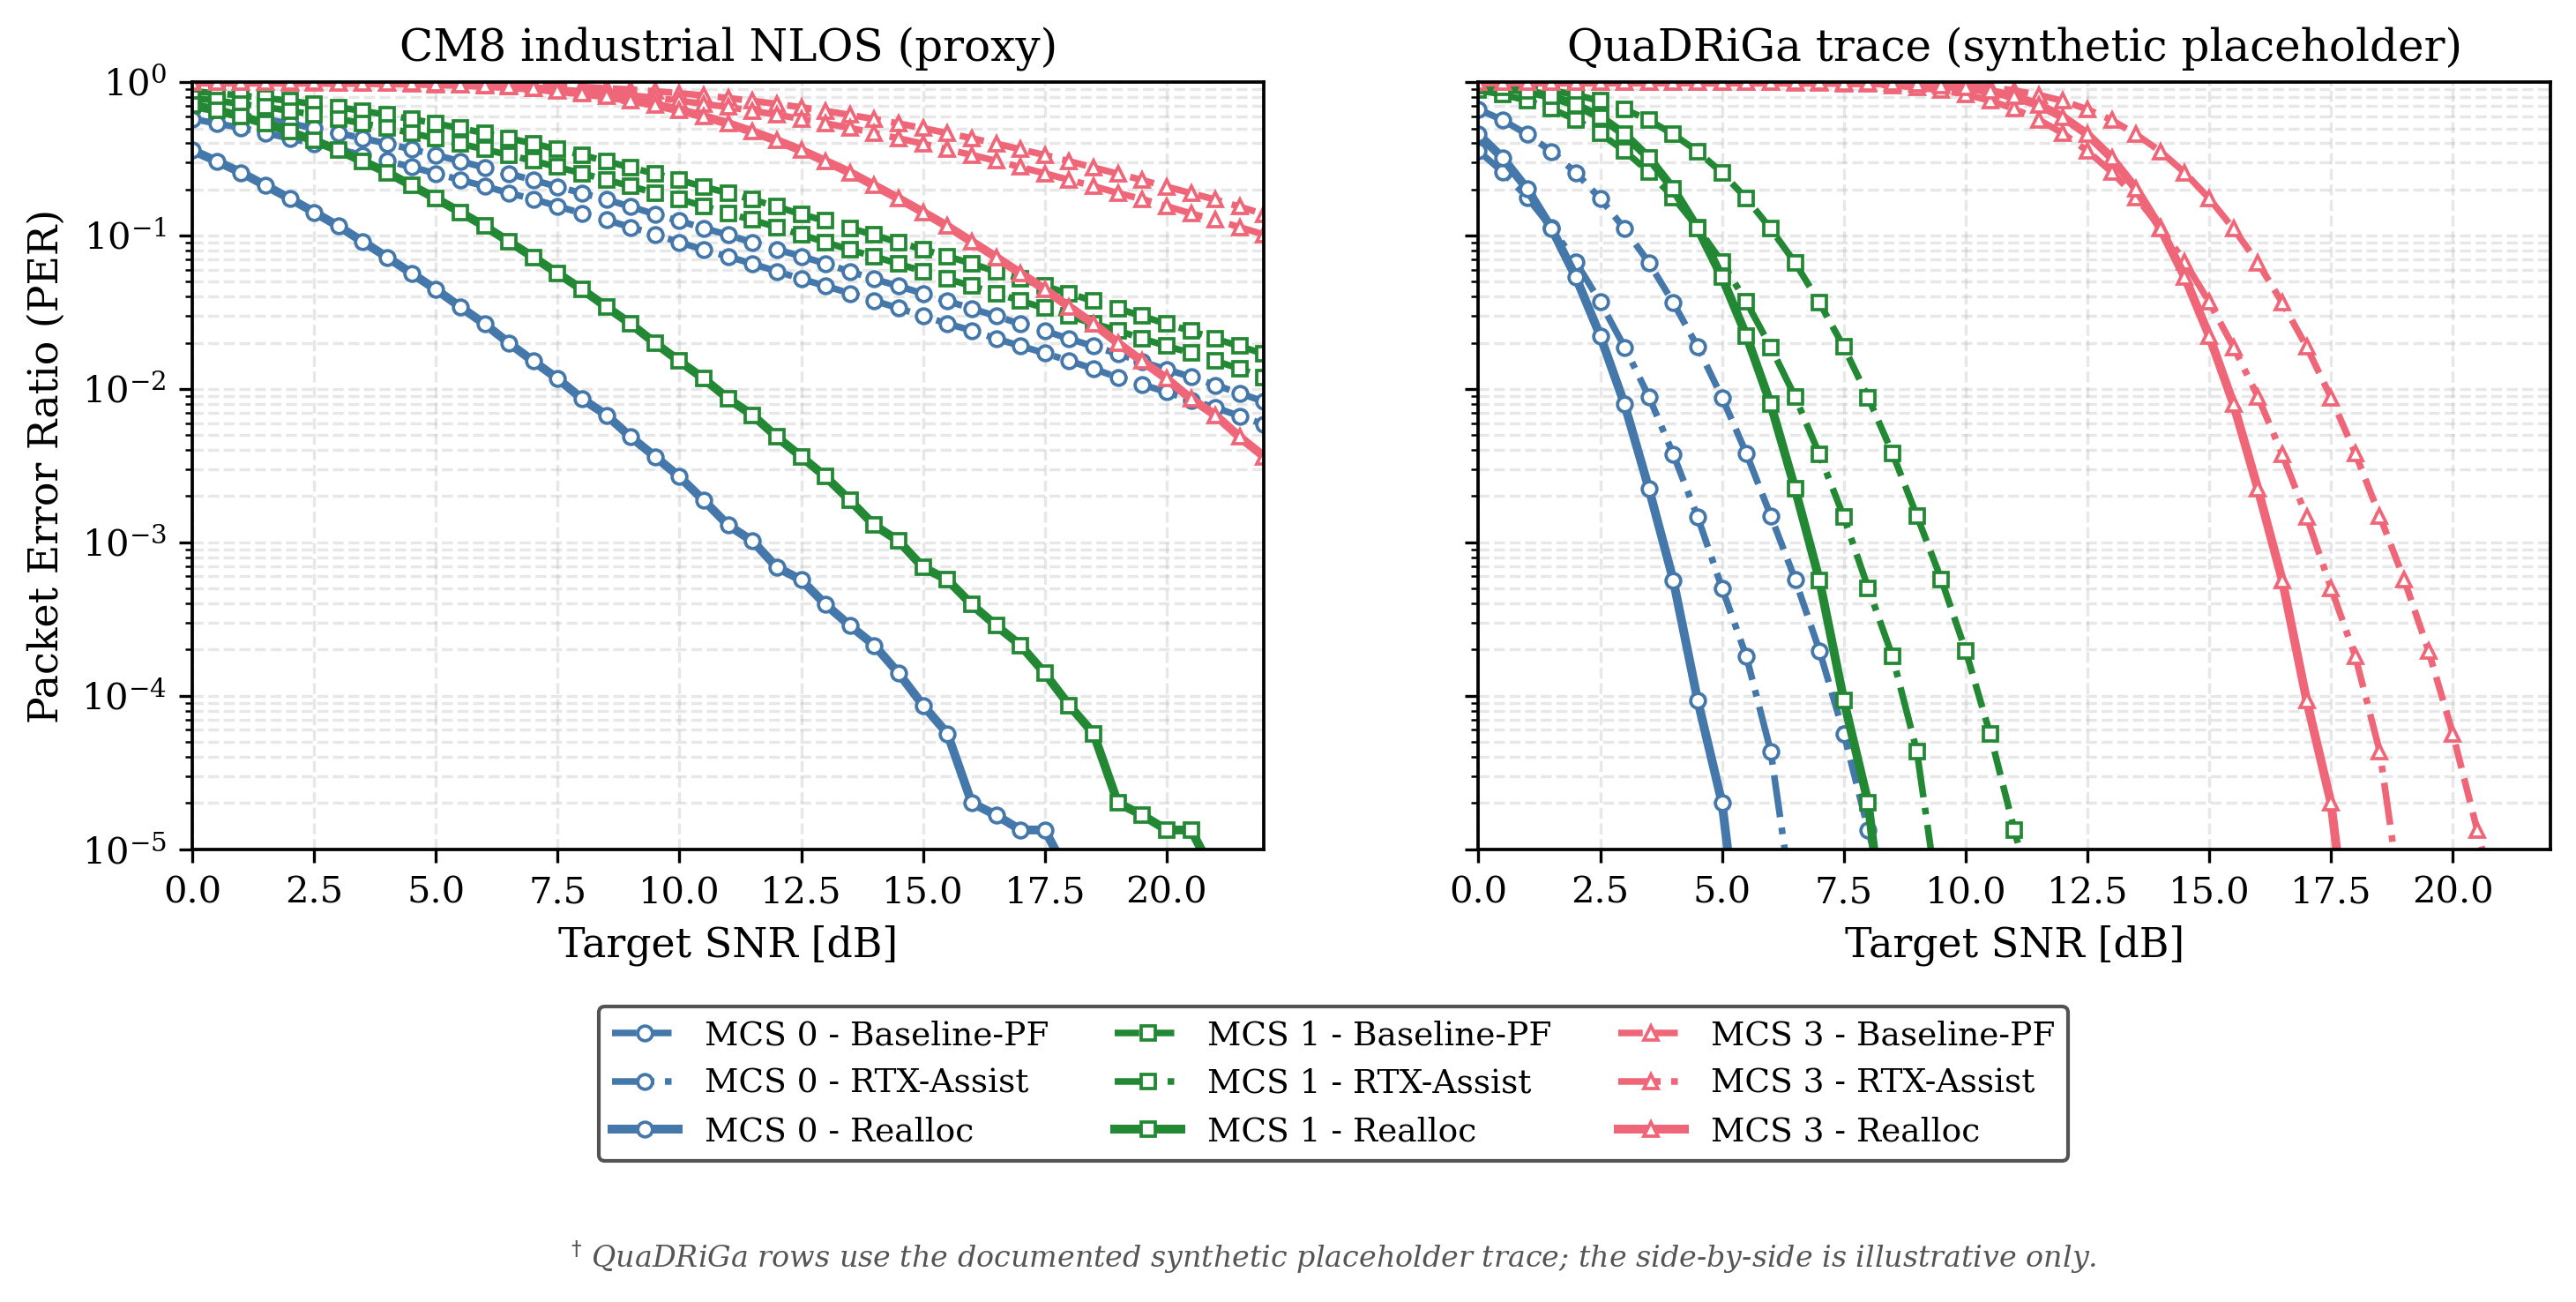
\includegraphics[width=0.95\columnwidth]{figs/fig_per_waterfall_quadriga_appendix.png}
  \caption{Side-by-side PER waterfall comparison between the CM8
  industrial NLOS proxy (left) and the QuaDRiGa-style ray-traced
  channel (right). \textbf{The QuaDRiGa rows use the synthetic
  placeholder trace shipped with the archive
  (\texttt{trace\_provenance=synthetic\_placeholder}) and must not
  be cited as measured industrial results.} The figure is reported
  in this appendix---rather than in the main results---precisely
  to keep the quantitative claims of
  Sections~\ref{sec:results-main}--\ref{sec:tab11} bound to the
  CM8 proxy. Replacement of the placeholder with a measured trace
  is mechanically enforced at run time by the simulator gate
  \texttt{-{}-requireMeasuredTrace=true}, which refuses to start
  a QuaDRiGa simulation whose provenance is anything other than
  \texttt{measured}.}
  \label{fig:per-waterfall-quadriga}
\end{figure}

\begin{figure}[t]
  \centering
  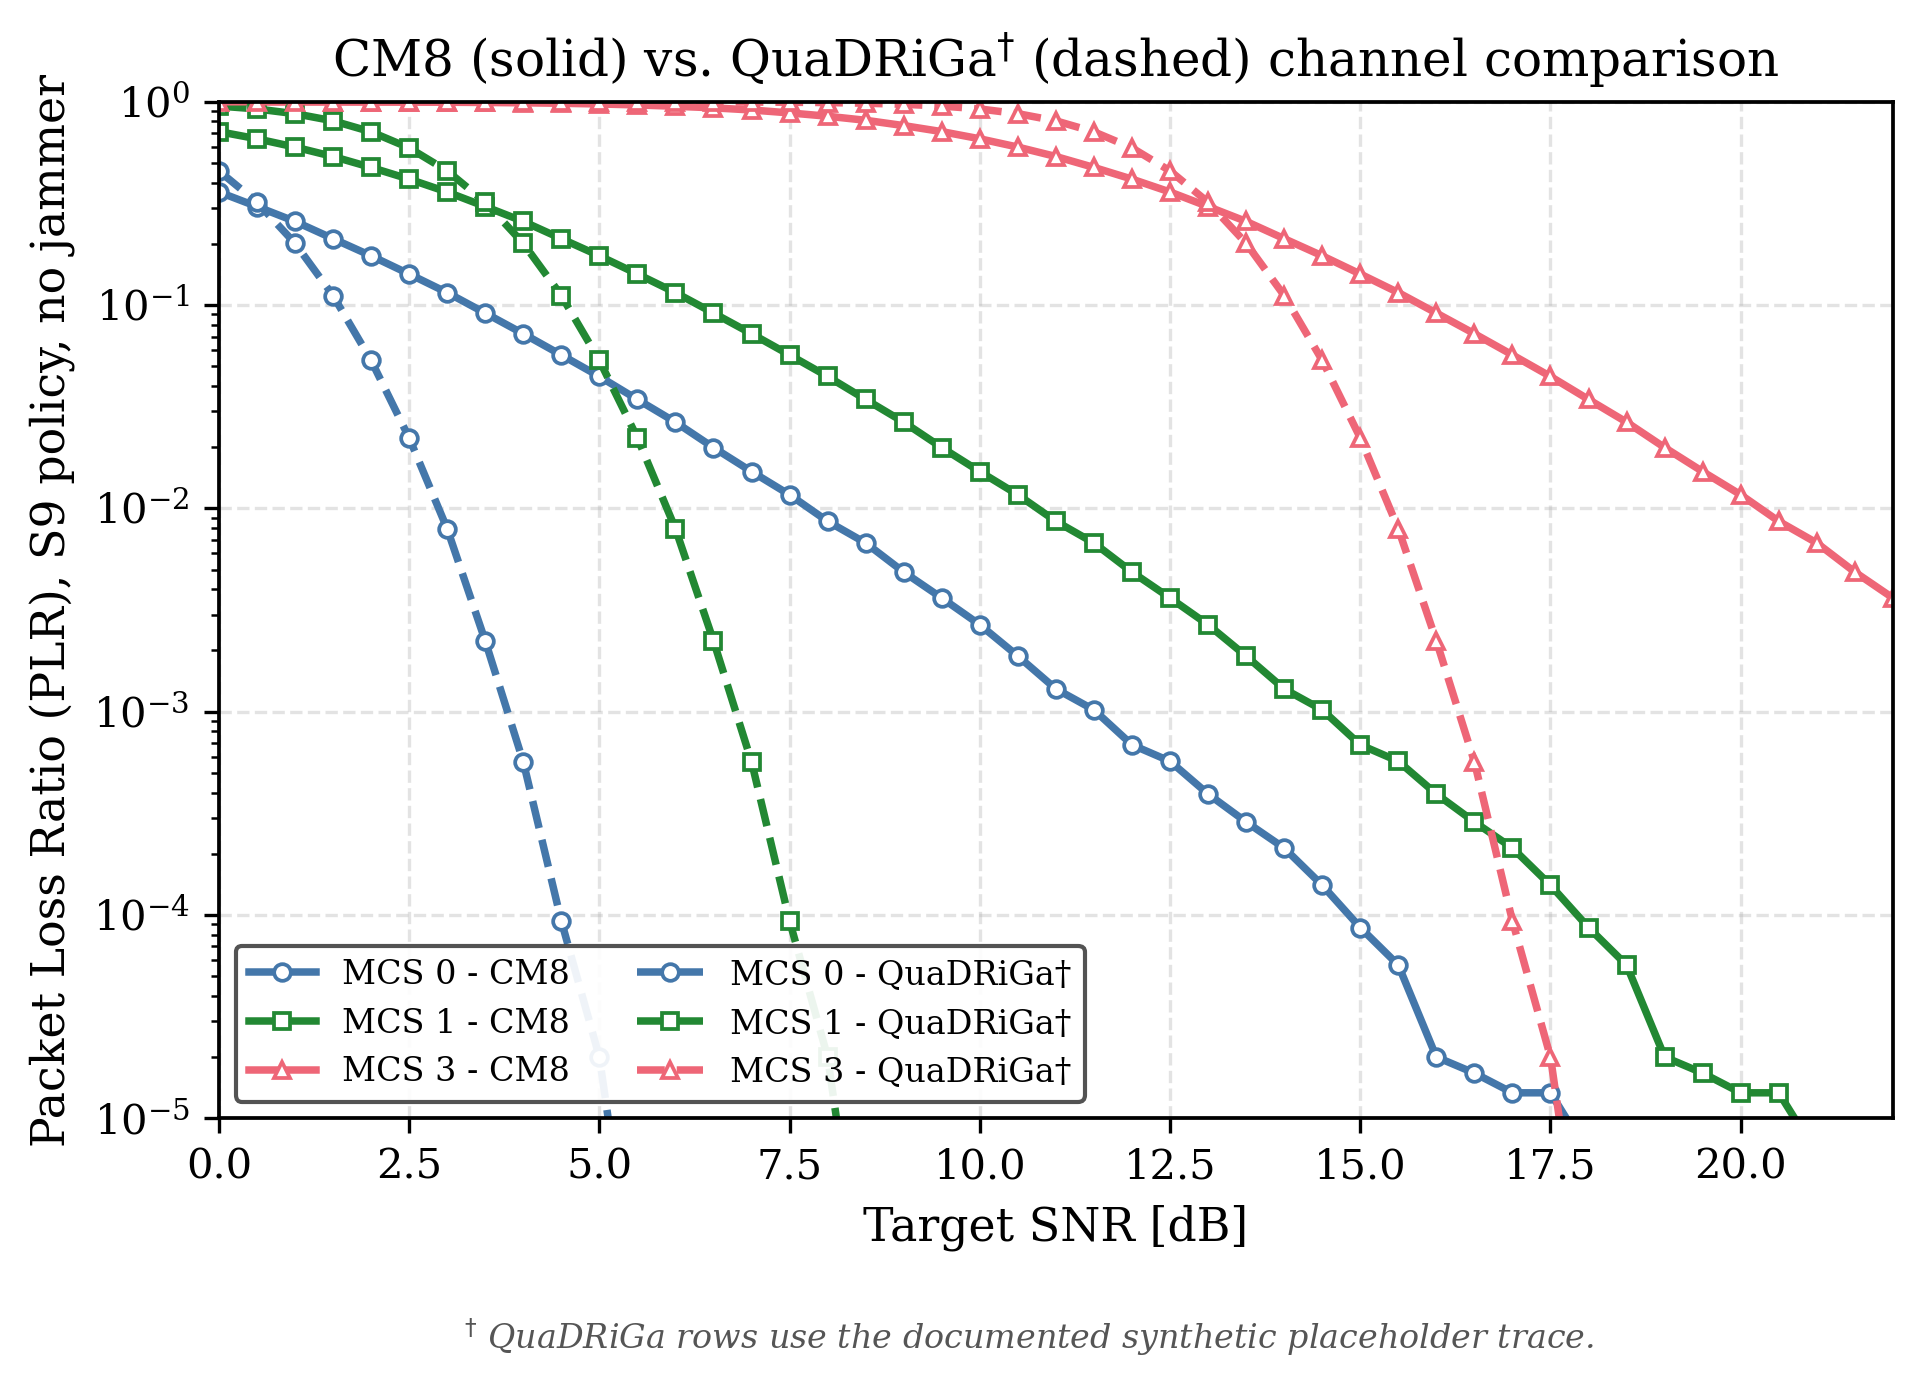
\includegraphics[width=0.95\columnwidth]{figs/fig_cm8_vs_quadriga.png}
  \caption{Channel-model comparison on the PLR axis at the S9
  policy operating point: CM8 stochastic model (solid) versus the
  QuaDRiGa-style ray-traced replay (dashed,
  $\dagger$-flagged). The CM8 curve is broader at the waterfall
  transition because it includes Rayleigh small-scale fading on
  top of log-normal shadowing; the QuaDRiGa curve is sharper
  because the trace-derived fading variance is narrower in the
  synthetic placeholder. The figure is intentionally relegated to
  this appendix and is \emph{not} used as quantitative evidence
  anywhere in the main paper.}
  \label{fig:cm8-quadriga-appendix}
\end{figure}

The two figures in this appendix expose the QuaDRiGa rows of the
campaign for reproducibility (the corresponding CSV rows are
released together with the code) but are not used in any
quantitative claim of this paper. The main-text policy
comparison, the S9 sensitivity sweep
(Section~\ref{sec:tab10}), the component ablation
(Section~\ref{sec:tab11}), the case study
(Section~\ref{sec:case-study-motion}) and the cross-validation
envelope (Section~\ref{sec:cross-validation}) all reference the
CM8 proxy rows only.

% =======================================================================
% Bibliography
% =======================================================================
\bibliographystyle{IEEEtran}
\bibliography{oj_ies}

\end{document}
